\documentclass[aspectratio=169]{beamer}
% Shared preamble for ml/ slide decks.
% Each lecture .tex starts with:
%   \documentclass[aspectratio=169]{beamer}
%   \input{../preamble}
% Compile from inside the chapter folder so \input{../preamble} resolves.

\usetheme{default}
\usecolortheme{dove}

\setbeamertemplate{navigation symbols}{}
\setbeamertemplate{footline}{%
  \hfill{\large\insertframenumber\,/\,\inserttotalframenumber}\hspace{0.8em}\vspace{0.5em}%
}

% Project palette (existing, kept for backwards compatibility with deferred/*)
\definecolor{popblue}{RGB}{52, 101, 164}
\definecolor{sampred}{RGB}{204, 0, 0}
\definecolor{paramgreen}{RGB}{0, 140, 70}
\definecolor{warnred}{RGB}{180, 40, 40}
\definecolor{orange1}{RGB}{220, 120, 0}
\definecolor{violet1}{RGB}{120, 50, 160}
\definecolor{lightbg}{RGB}{245, 245, 250}

% Armenian flag palette (use these for any 3-color highlight; per CLAUDE.md).
% "Nice versions": slightly de-saturated from the official spec for slide use,
% so they don't burn out under projector colors. Originals kept as *_pure.
\definecolor{armred}{RGB}{200, 30, 40}      % nice red (official #D90012 muted)
\definecolor{armblue}{RGB}{30, 70, 160}     % nice blue (official #0033A0 muted)
\definecolor{armorange}{RGB}{230, 160, 30}  % nice orange (official #F2A800 muted)
\definecolor{armred_pure}{HTML}{D90012}     % official Armenian flag red
\definecolor{armblue_pure}{HTML}{0033A0}    % official Armenian flag blue
\definecolor{armorange_pure}{HTML}{F2A800}  % official Armenian flag orange

\setbeamercolor{frametitle}{fg=popblue}
\setbeamercolor{title}{fg=popblue}

\usepackage{pgfplots}
\usepackage{tikz}
\usetikzlibrary{shapes, arrows.meta, positioning, calc, decorations.pathreplacing, patterns, matrix}
\pgfplotsset{compat=1.18}
\usepackage{amsmath, amssymb, amsfonts}
\usepackage{bm}
\usepackage{dsfont}
\usepackage{array}
\usepackage{pifont}
\usepackage{colortbl}
\usepackage{fontenc}

% Callout boxes. Purely additive - existing decks are unaffected.
% Usage: \begin{tcolorbox}[colback=armblue!8, colframe=armblue, boxrule=0.6pt, arc=2pt,
%                          title=\textbf{Key idea}] ... \end{tcolorbox}
% Palette convention (ml/SLIDE_STYLE.md): armblue=key idea, armred=trap/warning,
% paramgreen=takeaway or "Next", armorange=watch-out.
\usepackage[most]{tcolorbox}

% Cleaner table rules (\toprule, \midrule, \bottomrule). Also purely additive.
\usepackage{booktabs}

% \cancel{...} for struck-through terms in derivations (added 2026-08-11 for the
% importance-sampling frame in ch11_rl, where the dynamics cancel). Purely additive.
\usepackage{cancel}

% Minimal ML notation macros (subset of slds-lmu latex-math/basic-ml.tex).
% Kept here so we don't have to inline-expand every \thetav, \xv, etc.
% when porting upstream slides.
\newcommand{\R}{\mathds{R}}
\newcommand{\N}{\mathds{N}}
\newcommand{\E}{\mathds{E}}
\newcommand{\Xspace}{\mathcal{X}}
\newcommand{\Yspace}{\mathcal{Y}}
\newcommand{\Hspace}{\mathcal{H}}
\newcommand{\D}{\mathcal{D}}
\newcommand{\Dtrain}{\mathcal{D}_{\text{train}}}
\newcommand{\Dtest}{\mathcal{D}_{\text{test}}}
\newcommand{\xv}{\mathbf{x}}
\newcommand{\yv}{\mathbf{y}}
\newcommand{\Xmat}{\mathbf{X}}
\newcommand{\id}{\mathbf{I}}
\newcommand{\thetav}{\bm{\theta}}
\newcommand{\thetah}{\hat{\bm{\theta}}}
\newcommand{\lamv}{\bm{\lambda}}
\newcommand{\fx}{f(\xv)}
\newcommand{\fxt}{f(\xv \,|\, \bm{\theta})}
\newcommand{\fxi}{f\!\left(\xv^{(i)}\right)}
\newcommand{\fh}{\hat{f}}
\newcommand{\fxh}{\hat{f}(\xv)}
\newcommand{\yh}{\hat{y}}
\newcommand{\yih}{\hat{y}^{(i)}}
% \xi clashes with the Greek letter \xi; write \xv^{(i)} inline instead.
\newcommand{\yi}[1][i]{y^{(#1)}}
\newcommand{\xyi}[1][i]{\left(\xv^{(#1)},\, y^{(#1)}\right)}
\newcommand{\thx}{\bm{\theta}^\top \xv}
\newcommand{\sumin}{\sum_{i=1}^{n}}
\newcommand{\sumjp}{\sum_{j=1}^{p}}
\newcommand{\Lxy}{L\!\left(y, \fx\right)}
\newcommand{\Lxyi}{L\!\left(\yi, \fxi\right)}
\newcommand{\risk}{\mathcal{R}}
\newcommand{\riske}{\mathcal{R}_{\text{emp}}}
\newcommand{\risket}{\mathcal{R}_{\text{emp}}(\bm{\theta})}
\newcommand{\riskt}{\mathcal{R}(\bm{\theta})}
\newcommand{\riskr}{\mathcal{R}_{\text{reg}}}
\newcommand{\argmin}{\mathop{\mathrm{arg\,min}}}
\newcommand{\argmax}{\mathop{\mathrm{arg\,max}}}
\newcommand{\eps}{\varepsilon}


\usepackage{listings}
\lstset{
  basicstyle=\ttfamily\scriptsize,
  keywordstyle=\color{armblue}\bfseries,
  commentstyle=\color{paramgreen}\itshape,
  stringstyle=\color{armred},
  showstringspaces=false,
  language=Python,
  frame=single, framerule=0pt,
  backgroundcolor=\color{lightbg},
  numbers=none, breaklines=true, xleftmargin=4pt, xrightmargin=4pt,
}

\graphicspath{{fig/}{../00_shared/fig/}{../00_shared/fig/borrowed/}{../00_shared/fig/borrowed/3b1b/}{../../ml/13_rnns/fig/}}
\usetikzlibrary{tikzmark}

% ---- the equation, shown early and unpacked one piece at a time (2026-10-28) ----
% Pieces: Q popblue, K orange1, sqrt(d_k) violet1, softmax armred, V paramgreen. A preset lists the
% colours of Q, K^T, sqrt(d_k), softmax, V and the brackets; eqoff greys a piece out.
\colorlet{eqoff}{gray!40}
\newcommand{\attnd}[6]{{\color{#6}\textcolor{#4}{\mathrm{softmax}}\!\Big(\frac{\textcolor{#1}{Q}%
  \textcolor{#2}{K^{\top}}}{\textcolor{#3}{\sqrt{d_k}}}\Big)\,\textcolor{#5}{V}}}
\newcommand{\attni}[6]{{\color{#6}\textcolor{#4}{\mathrm{softmax}}(\textcolor{#1}{Q}%
  \textcolor{#2}{K^{\top}}/\textcolor{#3}{\sqrt{d_k}})\,\textcolor{#5}{V}}}
\newcommand{\pQK}{{popblue}{orange1}{eqoff}{eqoff}{eqoff}{eqoff}}
\newcommand{\pSM}{{eqoff}{eqoff}{eqoff}{armred}{eqoff}{eqoff}}
\newcommand{\pSQ}{{eqoff}{eqoff}{violet1}{eqoff}{eqoff}{eqoff}}
\newcommand{\pV}{{eqoff}{eqoff}{eqoff}{eqoff}{paramgreen}{eqoff}}
\newcommand{\pALL}{{popblue}{orange1}{violet1}{armred}{paramgreen}{black}}
\newcommand{\eqbig}[1]{\expandafter\attnd#1}
\newcommand{\eqsmall}[1]{\expandafter\attni#1}

% a milestone: the whole equation with one piece lit, before that piece is unpacked
\newcommand{\milestone}[3]{%
  \begin{frame}[plain]
    \vfill
    \begin{center}
      {\LARGE $\displaystyle\eqbig{#1}$}\\[1.4em]
      {\Large\bfseries\color{popblue} #2}\\[0.8em]
      \parbox{0.82\linewidth}{\centering\large #3}
    \end{center}
    \vfill
  \end{frame}}

% the small equation in the top-right corner of every titled frame of the current piece;
% \setpiece{\pQK} switches it on (or to another piece), \setpiece{} switches it off
\def\curpiece{}   % \def, not \newcommand: a \long macro never \ifx-matches \empty
\newcommand{\setpiece}[1]{\xdef\curpiece{#1}}
\addtobeamertemplate{frametitle}{}{%
  \ifx\curpiece\empty\else
    \begin{tikzpicture}[remember picture, overlay]
      \node[anchor=north east, inner sep=2pt, font=\footnotesize]
        at ([shift={(-0.25cm,-0.22cm)}]current page.north east) {$\eqsmall{\curpiece}$};
    \end{tikzpicture}%
  \fi}

% callout boxes, matching LLM-1, LLM-2 and LLM-6
\newcommand{\keybox}[1]{\fcolorbox{armblue}{armblue!8}{\parbox{0.97\linewidth}{\small #1}}}
\newcommand{\trapbox}[1]{\fcolorbox{armred}{armred!8}{\parbox{0.97\linewidth}{\small #1}}}
\newcommand{\takebox}[1]{\fcolorbox{paramgreen}{paramgreen!8}{\parbox{0.97\linewidth}{\small #1}}}
\newcommand{\watchbox}[1]{\fcolorbox{armorange}{armorange!12}{\parbox{0.97\linewidth}{\small #1}}}

\newcommand{\sectiontransition}[2]{%
  \begin{frame}[plain]
    \vfill
    \begin{center}
      {\Huge\bfseries\color{popblue} #1}\\[1.1em]
      {\large #2}
    \end{center}
    \vfill
  \end{frame}}

% small credit / citation lines
\newcommand{\bbb}{{\scriptsize\color{gray} 3Blue1Brown}}
\newcommand{\lmu}{{\scriptsize\color{gray} Source: LMU I2DL (slds-lmu), CC BY 4.0}}
\newcommand{\paper}[1]{{\scriptsize\color{gray} #1}}
\newcommand{\src}[1]{{\scriptsize\color{gray} #1}}
\newcommand{\link}[2]{\href{#1}{\textcolor{popblue}{#2}}}   % no underline: long titles must break

% full-bleed 3Blue1Brown still with a one-line caption pinned near the bottom. Wrapped in a group
% so the background template reverts after this one [plain] frame. Needs 2 pdflatex passes.
\newcommand{\bbbcap}[2]{%
  {\usebackgroundtemplate{\includegraphics[width=\paperwidth,height=\paperheight]{#1}}%
  \begin{frame}[plain]
    \begin{tikzpicture}[remember picture, overlay]
      \node[anchor=south west, font=\tiny, text=white!60]
        at ([shift={(0.26cm,0.16cm)}]current page.south west) {3Blue1Brown};
      \node[anchor=south, font=\small\itshape, text=white, fill=black!60,
            inner sep=5pt, rounded corners, text width=0.86\paperwidth, align=center]
        at ([shift={(0,0.85cm)}]current page.south) {#2};
    \end{tikzpicture}
  \end{frame}}%
}

\title{Attention}
\subtitle{How tokens share meaning}
\date{}

\begin{document}

\begin{frame}[plain]
  \titlepage
  \begin{center}\scriptsize\color{gray}
    LLM chapter, session 3. Parts adapt LMU I2DL (CC BY 4.0) and 3Blue1Brown, ``Deep Learning''
    chapters 5 and 6.
  \end{center}
\end{frame}

% ============================================================ LINKS (2026-10-27, as in LLM-1 and LLM-2)
\begin{frame}{Before we start: two videos and a demo}
  \begin{columns}[T]
    \column{0.49\textwidth}
    \keybox{\raggedright\textbf{Recommended viewing}\\[4pt]
    3Blue1Brown, \link{https://www.youtube.com/watch?v=eMlx5fFNoYc}{Attention in transformers,
    step-by-step \textbar{} Deep Learning Chapter 6} (2024, 26 min): today's lecture, animated.
    Many stills in this deck are from it.\\[6pt]
    Andrej Karpathy, \link{https://youtu.be/kCc8FmEb1nY?t=2533}{Let's build GPT: from scratch, in
    code, spelled out.} (2023). From 42:13: attention built in code, one version at a time; why
    divide by $\sqrt{d_k}$ at 1:16:56.}
    \column{0.49\textwidth}
    \takebox{\raggedright\textbf{Live demo:}
    \link{https://poloclub.github.io/transformer-explainer/}{Transformer Explainer}\\[4pt]
    GPT-2 small running in your browser (about a 600 MB download): type a sentence, open one of the
    12 heads, watch $QK^\top$, softmax and the weights.}
    \vskip 4pt
    {\small\textbf{Try:}}
    \begin{itemize}\small
      \item our creature sentence: does a head send creature to fluffy?
      \item a sentence with ``it'': which head finds what ``it'' is?
      \item the same head on two different sentences
    \end{itemize}
  \end{columns}
\end{frame}

% ================================================================
% WHERE WE ARE - the chapter map (py_src/llm_roadmap.py)
\begin{frame}{Where we are: one forward pass}
  \begin{center}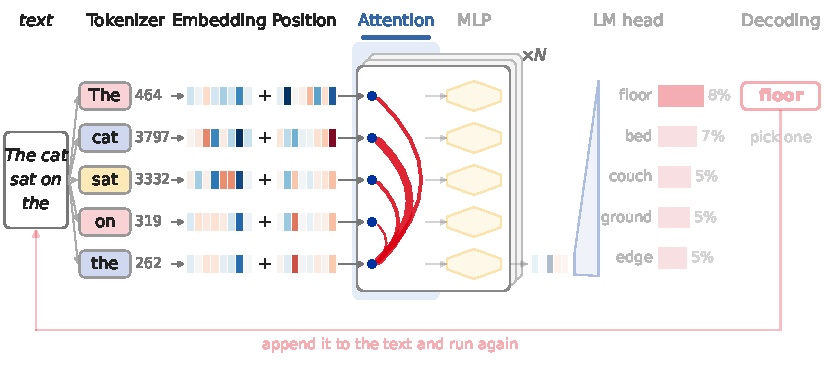
\includegraphics[width=\linewidth]{roadmap_attention_pass.pdf}\end{center}
  \vskip -2pt
  {\small Today: the \textbf{attention} step - how each token's vector picks up meaning from the
  other tokens.}
\end{frame}

\begin{frame}{Where we are: the life of a model}
  \begin{center}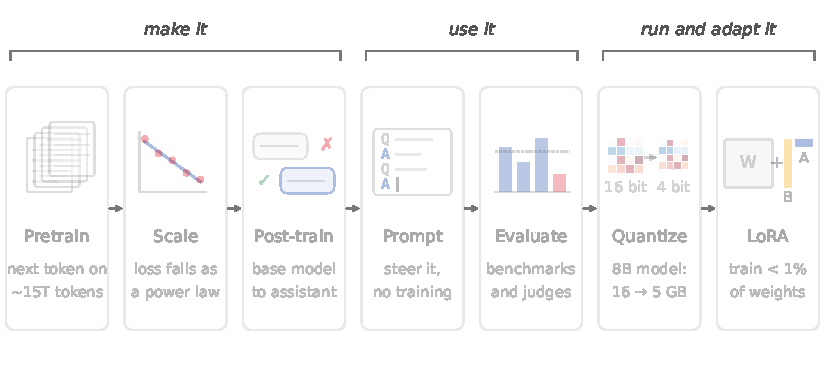
\includegraphics[width=\linewidth]{roadmap_attention_life.pdf}\end{center}
  \vskip -2pt
  {\small Later: where these weights come from, and what you do with them once you have them.}
\end{frame}

% ================================================================
% COLD OPEN - L21's two walls
\begin{frame}{[54] left two walls}
  \begin{columns}[T]
    \column{0.55\textwidth}
      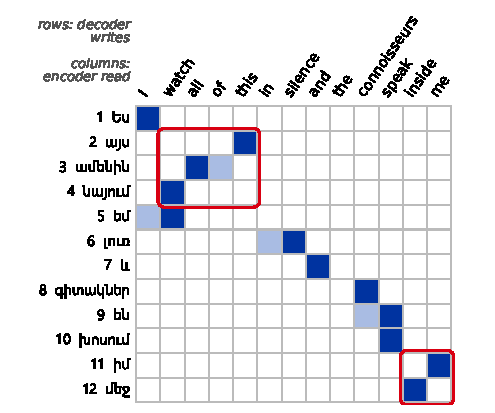
\includegraphics[width=\linewidth]{alignment_grid_1.pdf}
    \column{0.43\textwidth}
      \small
      \textbf{Wall 1: one $C$ for every step.} The decoder writes the Armenian line one word per
      row. Each row needs one or two \emph{different} English words, and seq2seq hands every row
      the same context vector $C$.
      \vskip 6pt
      \textbf{Wall 2: the queue.} The RNN reads one token after another: 1{,}000 tokens are
      1{,}000 steps in a row, while most of the GPU waits.
      \vskip 10pt
      \keybox{\textbf{Predict:} how would you fix wall 1? What should row 4 (``watch'') get
      instead of $C$?}
  \end{columns}
\end{frame}

\begin{frame}{The fix, in one idea}
  \begin{columns}[T]
    \column{0.52\textwidth}
    Don't force everything through one vector. At \textbf{each} output step, let the decoder
    \textbf{look back over every input state} and take a \emph{weighted average}: heavy weight on
    the words this step needs, light weight on the rest.
    \vskip 8pt
    Row 4 (``watch'') puts most of its weight on ``watch''; row 5 picks a different mix. Every
    step gets its own context.
    \vskip 8pt
    \takebox{That weighted look-back \emph{is} \textbf{attention}. Today unpacks this one sentence,
    and then takes it much further.}
    \column{0.46\textwidth}
    \begin{center}
      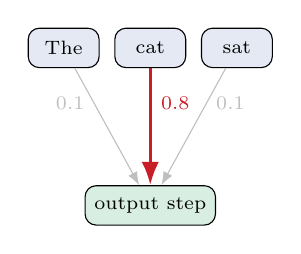
\begin{tikzpicture}[font=\scriptsize, >=Latex,
        e/.style={draw, rounded corners, minimum width=0.9cm, minimum height=0.5cm, fill=armblue!12},
        d/.style={draw, rounded corners, minimum width=1.1cm, minimum height=0.5cm, fill=paramgreen!15}]
        \foreach \i/\w in {0/The,1/cat,2/sat} \node[e] (h\i) at (\i*1.1,2) {\w};
        \node[d] (dec) at (1.1,0) {output step};
        \draw[->, gray!50] (h0)--(dec) node[pos=0.3,left,font=\scriptsize]{0.1};
        \draw[->, very thick, armred] (h1)--(dec) node[pos=0.3,right,font=\scriptsize,text=armred]{0.8};
        \draw[->, gray!50] (h2)--(dec) node[pos=0.3,right,font=\scriptsize]{0.1};
      \end{tikzpicture}\\[4pt]
      {\footnotesize weights sum to 1; this step leans on ``cat''}
    \end{center}
  \end{columns}
\end{frame}

% the destination: the whole equation up front, each piece with the question it answers
\begin{frame}{Where we are going: one line}
  \vskip 30pt
  \begin{center}
  {\LARGE $\displaystyle
    \tikzmarknode{dsm}{\textcolor{armred}{\mathrm{softmax}}}\!\Big(\frac{\tikzmarknode{dqk}{%
    \textcolor{popblue}{Q}\textcolor{orange1}{K^{\top}}}}{\tikzmarknode{dsq}{\textcolor{violet1}{%
    \sqrt{d_k}}}}\Big)\,\tikzmarknode{dv}{\textcolor{paramgreen}{V}}$}
  \end{center}
  \begin{tikzpicture}[remember picture, overlay, font=\small, >=Latex]
    \node[text=popblue] (a) at ([shift={(2.4cm,1.15cm)}]dqk.north) {who matches whom?};
    \draw[->, popblue, thick] (a.west) -- (dqk.north east);
    \node[text=armred] (b) at ([shift={(-2.0cm,1.15cm)}]dsm.north) {why this function?};
    \draw[->, armred, thick] (b.south) -- (dsm.north);
    \node[text=violet1] (c) at ([shift={(-2.6cm,-0.95cm)}]dsq.south) {why divide by this?};
    \draw[->, violet1, thick] (c.east) -- (dsq.south west);
    \node[text=paramgreen] (d) at ([shift={(2.0cm,-0.95cm)}]dv.south) {what gets handed over?};
    \draw[->, paramgreen, thick] (d.north) -- (dv.south);
  \end{tikzpicture}
  \vskip 52pt
  \keybox{This line is the whole of today. By the end, every piece of it has a job you can
  explain. Walls 1 and 2 say why the line exists at all; then we take it apart one piece at a
  time, and finally see what the model may \emph{not} look at: the mask.}
\end{frame}

\begin{frame}{Outline}
  \tableofcontents
\end{frame}

% ================================================================
\section{Wall 1: look back}
\sectiontransition{Wall 1: look back}{A different context for every word you write.}

\begin{frame}{Score, softmax, weighted sum}
  At each output step, attention does three things. The step from the fix, as a picture:
  \vskip 2pt
  \begin{center}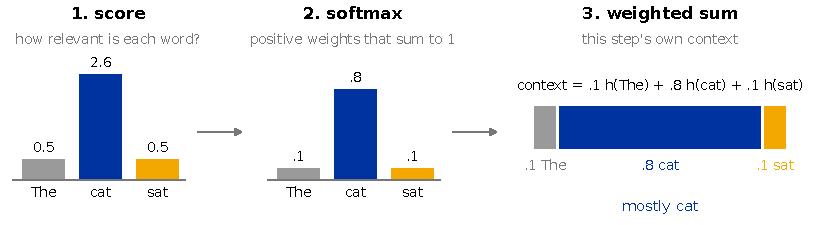
\includegraphics[width=\linewidth]{att_three_moves.pdf}\end{center}
  \vskip -4pt
  {\small The blend is this step's own context, its personal $C$. The decoder's current state
  does the asking, the encoder's states answer. The score itself: Bahdanau et al.\ fed the two
  states to a small learned network; later models just take their dot product, as we will.}
  \vskip 6pt
  \keybox{You have seen the three moves: LLM-2 ran them by hand on ``dog bites man'', and softmax
  and weighted sums are [41]. The new part is \emph{what} gets scored and blended.}
\end{frame}

\begin{frame}{Learned, not drawn}
  \begin{columns}[T]
    \column{0.54\textwidth}
    \begin{center}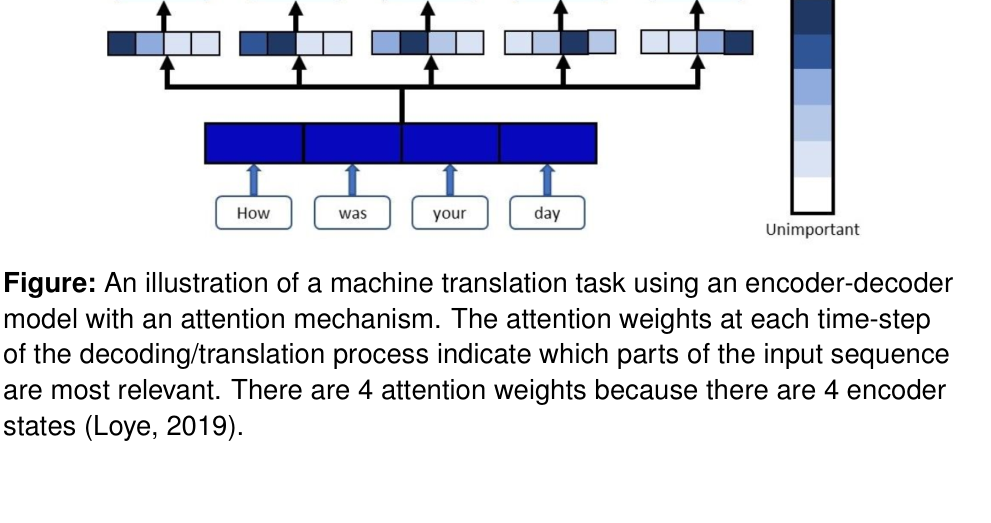
\includegraphics[width=0.84\linewidth]{lmu_translation_attention.png}\end{center}
    {\scriptsize Translation: at each output step the model learns its own weights over the input
    words (the bar on the right). \paper{(Bahdanau, Cho \& Bengio, 2015: the first attention)}}
    \column{0.44\textwidth}
    \begin{center}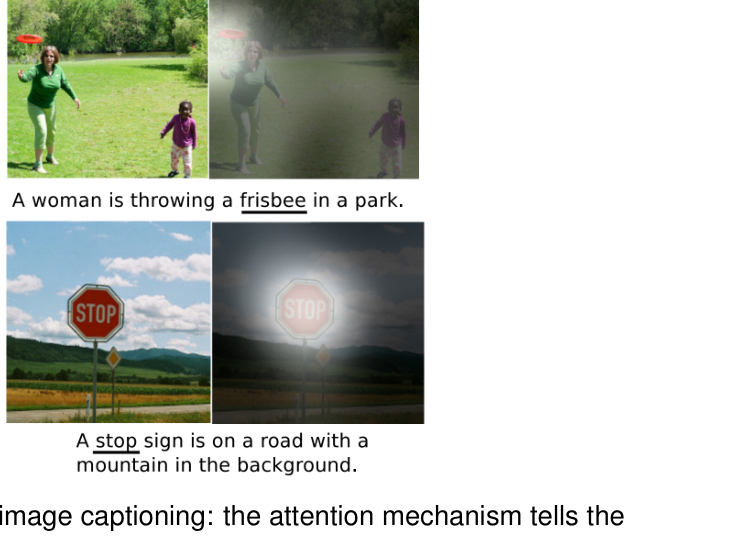
\includegraphics[width=0.46\linewidth, trim=0 53 322 0, clip]{lmu_captioning_attention.png}\end{center}
    {\scriptsize Captioning: weights over \emph{pixels} while writing each word.
    \paper{(Xu et al., 2015)}}
  \end{columns}
  \vskip 2pt
  \takebox{Stack the steps and you get a grid like [54]'s, drawn by training, not by hand: nobody
  labels the alignments, only the translation loss trains them. Wall 1 is down.}
  \vskip 1pt \lmu
\end{frame}

% ================================================================
\section{Wall 2: drop the queue}
\sectiontransition{Wall 2: drop the queue}{If every word can look at every word, who needs the
recurrence?}

\begin{frame}{The encoder still reads one word at a time}
  \begin{columns}[T]
    \column{0.55\textwidth}
    Attention took down wall 1: every output step gets its own mix of the encoder's states.
    \vskip 6pt
    But those states are still built by an RNN, one after another: $z_2$ waits for $z_1$, $z_3$
    waits for $z_2$. Wall 2 is still standing.
    \vskip 10pt
    \keybox{\textbf{Predict:} attention lets any position read any other position directly.
    Could it build the vectors themselves, with no recurrence at all?}
    \column{0.43\textwidth}
    \vskip 14pt
    \begin{center}
      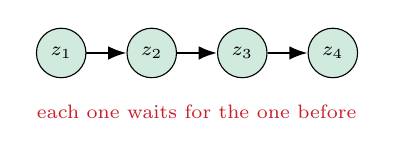
\begin{tikzpicture}[font=\scriptsize, >=Latex,
          n/.style={draw, circle, minimum size=0.62cm, fill=paramgreen!18}]
        \foreach \i/\x in {1/0,2/1.15,3/2.3,4/3.45} \node[n] (z\i) at (\x,0) {$z_{\i}$};
        \foreach \a/\b in {1/2,2/3,3/4} \draw[->, thick] (z\a) -- (z\b);
        \node[armred] at (1.72,-0.75) {each one waits for the one before};
      \end{tikzpicture}
    \end{center}
  \end{columns}
\end{frame}

\begin{frame}{Words need their own sentence}
  \begin{columns}[T]
    \column{0.5\textwidth}
    \begin{center}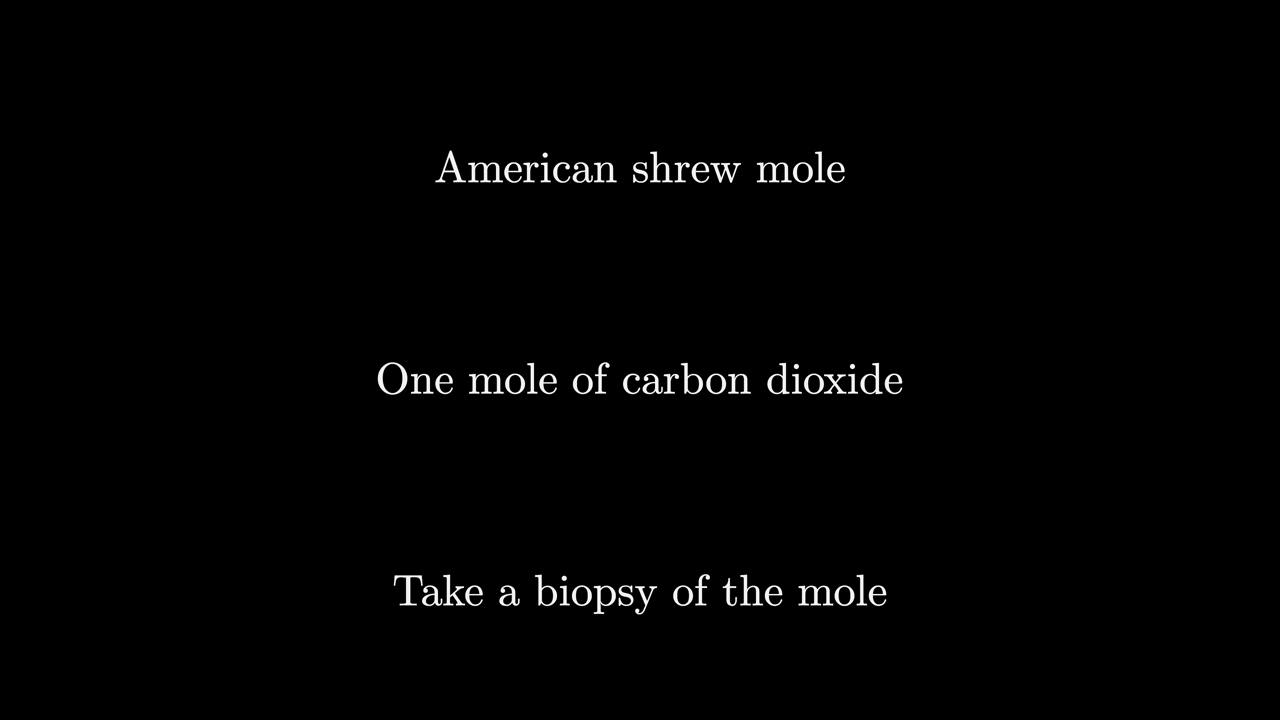
\includegraphics[width=0.9\linewidth]{mole_polysemy.png}\end{center}
    {\scriptsize ``mole'' means three different things, but the vector it starts with - its row
    of the table (LLM-2) - is identical in all three.}
    \column{0.5\textwidth}
    \begin{center}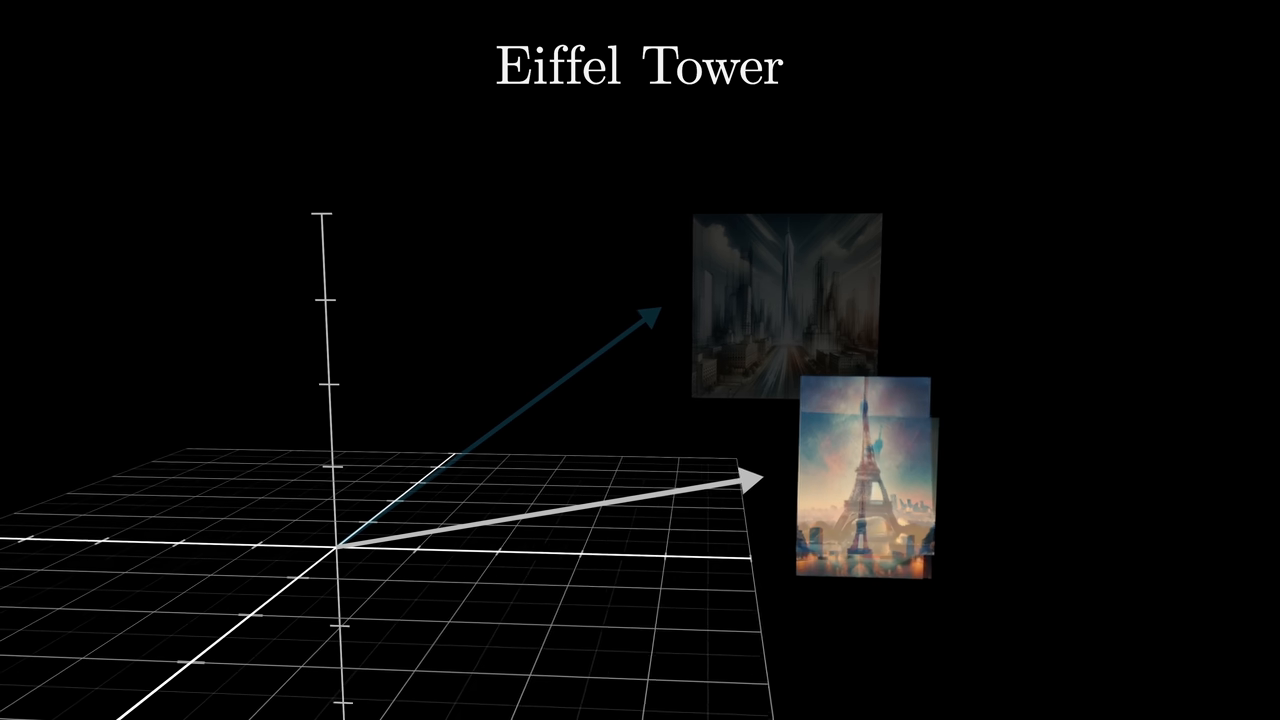
\includegraphics[width=0.9\linewidth]{eiffel_context.png}\end{center}
    {\scriptsize ``tower'', after ``Eiffel'', should move toward Paris, France, steel.}
  \end{columns}
  \vskip 3pt
  \keybox{Same with ``a machine learning \textbf{model}'' and ``a fashion \textbf{model}''. Each
  word's vector has to change with its sentence, and what it needs is in that same sentence.}
  \vskip 1pt \bbb
\end{frame}

% the murder-mystery still: the last vector has to carry the whole story
\bbbcap{fs_mystery.jpg}{To fill the blank, the \emph{last} vector must have soaked up the whole
story.}

\begin{frame}{The sentence talks to itself}
  \begin{columns}[T]
    \column{0.55\textwidth}
    In translation the \emph{decoder's} state did the asking and the \emph{encoder's} states
    answered: two sequences.
    \vskip 6pt
    In \textbf{self}-attention the asking and the answering both come from the \textbf{same}
    sentence. Every word asks, and every word answers. One round is all-to-all messaging: each word gathers what it needs
    from all the others.
    \vskip 8pt
    \fcolorbox{armred}{armred!8}{\parbox{0.95\linewidth}{\small
      So yes to the predict: each word's new vector is built from all the others in one step, and
      the recurrence goes. The 2017 paper said it in its title: \textbf{``Attention Is All You
      Need.''} \paper{(Vaswani et al., 2017)}}}
    \column{0.43\textwidth}
    \begin{center}
      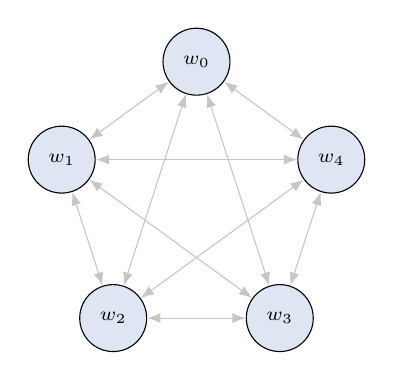
\begin{tikzpicture}[font=\scriptsize,>=Latex]
        \foreach \i/\a in {0/90,1/162,2/234,3/306,4/18}
          \node[draw,circle,fill=armblue!14,minimum size=0.85cm] (w\i) at (\a:1.8) {$w_{\i}$};
        \foreach \i in {0,...,4}\foreach \j in {0,...,4}{\ifnum\i<\j \draw[gray!45,<->](w\i)--(w\j);\fi}
      \end{tikzpicture}\\[4pt]
      {\footnotesize every word attends to every word}
    \end{center}
  \end{columns}
\end{frame}

\begin{frame}{Sequential vs.\ all-to-all}
  \begin{center}
    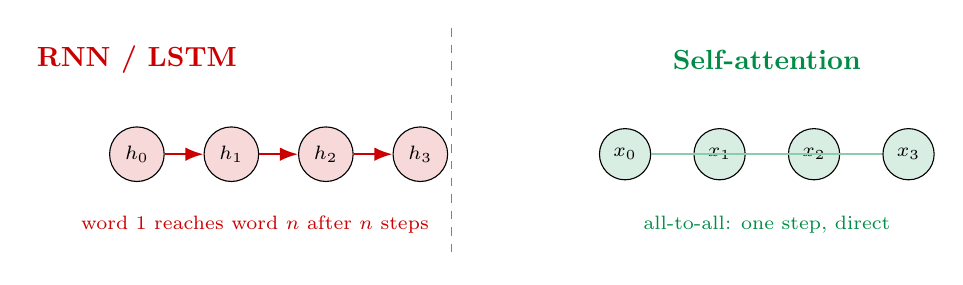
\begin{tikzpicture}[font=\scriptsize, >=Latex]
      \node[font=\normalsize\bfseries, text=sampred] at (-4,2.9) {RNN / LSTM};
      \foreach \i/\y in {0/-4.0,1/-2.8,2/-1.6,3/-0.4}
        \node[draw, circle, fill=sampred!15, minimum size=0.55cm] (l\i) at (\y,1.7) {$h_\i$};
      \draw[->,thick,sampred] (l0)--(l1); \draw[->,thick,sampred] (l1)--(l2); \draw[->,thick,sampred] (l2)--(l3);
      \node[text=sampred] at (-2.5,0.8) {word 1 reaches word $n$ after $n$ steps};
      \node[font=\normalsize\bfseries, text=paramgreen] at (4,2.9) {Self-attention};
      \foreach \i/\y in {0/2.2,1/3.4,2/4.6,3/5.8}
        \node[draw, circle, fill=paramgreen!15, minimum size=0.55cm] (t\i) at (\y,1.7) {$x_\i$};
      \foreach \a/\b in {0/1,0/2,0/3,1/2,1/3,2/3} \draw[paramgreen!45,thick] (t\a)--(t\b);
      \node[text=paramgreen] at (4,0.8) {all-to-all: one step, direct};
      \draw[dashed,gray] (0,3.3)--(0,0.4);
    \end{tikzpicture}
  \end{center}
  \vskip 4pt
  \begin{center}
  \fcolorbox{popblue}{popblue!6}{\parbox{0.8\linewidth}{\centering\small
    Three wins: \textbf{parallel} (all tokens at once) $\cdot$ \textbf{direct} (any token to any
    other) $\cdot$ \textbf{contextual} (each vector changes with its sentence). And it is all
    matrix products: the work a GPU is built for ([40], [54]'s second wall).}}
  \end{center}
  \vskip 2pt
  \watchbox{And word order? Self-attention alone cannot see it (LLM-2's ``dog bites man''). That
  is why the position information goes into the vectors \emph{before} the first attention layer.}
\end{frame}

\begin{frame}{The paper behind the title}
  \begin{itemize}
    \item Vaswani et al.\ (2017): eight authors at Google, and a footnote that reads ``Equal
      contribution. Listing order is random.'' Its main results were in machine translation.
    \item The title was Llion Jones's idea, after the Beatles' ``All You Need Is Love''. The name
      ``Transformer'' was there from day zero; Jakob Uszkoreit had two Transformer toys as a kid.
    \item All eight later left Google and founded or joined companies: Cohere, Character.AI,
      Sakana AI, among others. One came back: Noam Shazeer returned in 2024.
    \item Google Scholar today: about \textbf{279,000} citations. Within a year the block powered
      GPT and BERT (LLM-5).
  \end{itemize}
  \vskip 6pt
  \takebox{A translation paper that set out to drop the recurrence. Attention is the part that
  stayed.}
  \vskip 2pt
  \src{Wired (Levy, 20 March 2024), ``8 Google Employees Invented Modern AI. Here's the Inside
  Story''; the paper's footnote; Google Scholar, read 27 Oct 2026 (278,670).}
\end{frame}

% ================================================================
\section{One head, slowly}
\sectiontransition{One head, slowly}{Every piece of the equation, and why it is there.}

\begin{frame}{The goal, made concrete}
  \begin{columns}[T]
    \column{0.5\textwidth}
    \begin{center}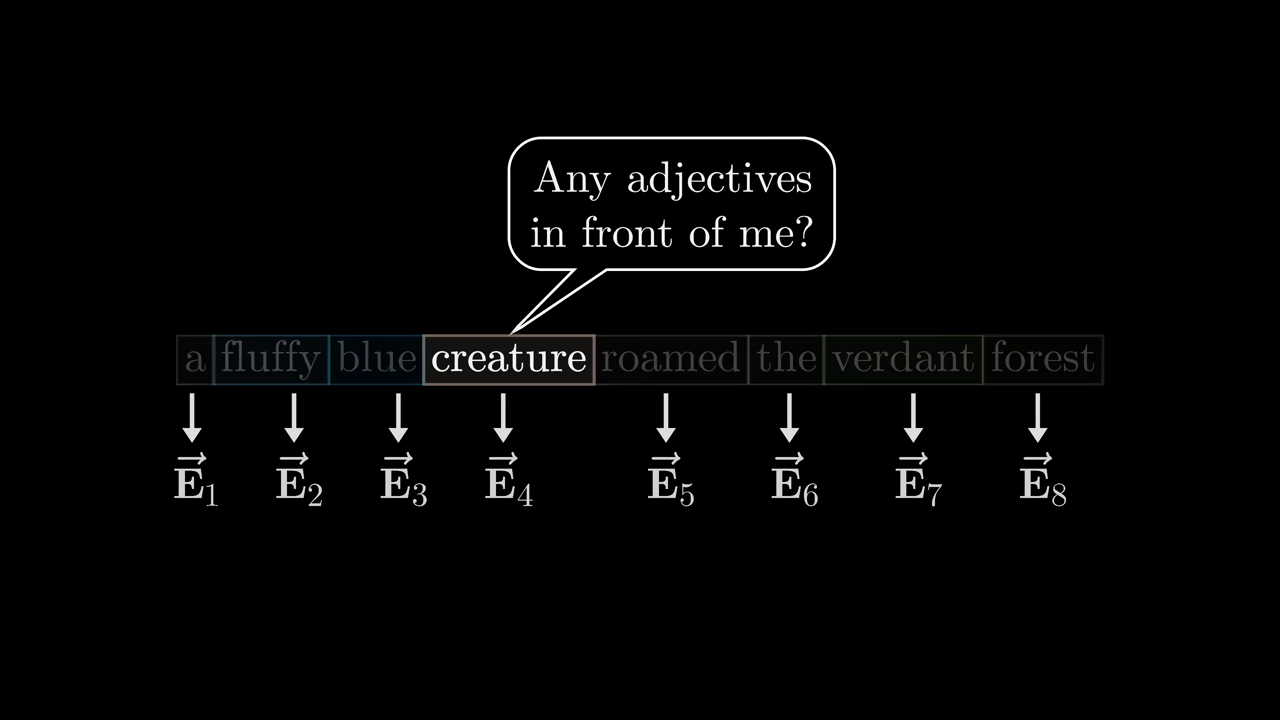
\includegraphics[width=\linewidth]{query_creature.png}\end{center}
    \column{0.5\textwidth}
    Sentence: \emph{``a fluffy blue creature roamed the verdant forest.''}
    \vskip 6pt
    We want the noun \textbf{creature} to absorb its adjectives \textbf{fluffy} and
    \textbf{blue}, so its vector means \emph{``a fluffy, blue creature.''}
    \vskip 6pt
    Two questions the mechanism must answer:
    \begin{itemize}\small
      \item Which words are \textbf{relevant} to creature?
      \item \textbf{What} should they hand over?
    \end{itemize}
  \end{columns}
  \vskip 1pt \bbb
\end{frame}

\begin{frame}{Predict first: who does ``creature'' listen to?}
  \begin{columns}[T]
    \column{0.47\textwidth}
    Toy vectors with 4 numbers, read as [adjective, fluffy, blue, noun]. A darker cell is a
    bigger number.
    \vskip 6pt
    No learned matrices yet: each vector is its own query, its own key and its own value, the
    simplified version from LLM-2. Score = dot product divided by $\sqrt{4} = 2$; softmax by rows;
    weighted sum.
    \column{0.51\textwidth}
    \vskip 4pt
    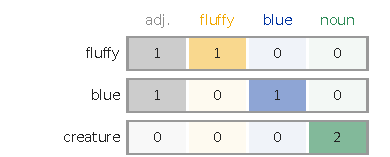
\includegraphics[width=\linewidth]{att_toy_chips.pdf}
  \end{columns}
  \vskip 12pt
  \keybox{\textbf{Predict:} which of the three words gets the biggest share of creature's
  attention?}
\end{frame}

\begin{frame}{Itself}
  \begin{columns}[T]
    \column{0.48\textwidth}
    \small
    creature $\cdot$ creature $= 4$, so its own score is $4/2 = 2$; against fluffy and blue it
    scores $0$.
    \vskip 4pt
    Weights $0.107,\ 0.107,\ \mathbf{0.787}$: creature spends \textbf{79\%} of its attention on
    itself. Its update:
    \[ 0.107\,(1,1,0,0) + 0.107\,(1,0,1,0) \]
    \[ {}+ 0.787\,(0,0,0,2) = (0.21,\ 0.11,\ 0.11,\ 1.57) \]
    Mostly more creature. And the \textbf{scores} are symmetric: fluffy $\cdot$ blue $=$ blue
    $\cdot$ fluffy (softmax runs row by row, so the weights can still differ).
    \column{0.5\textwidth}
    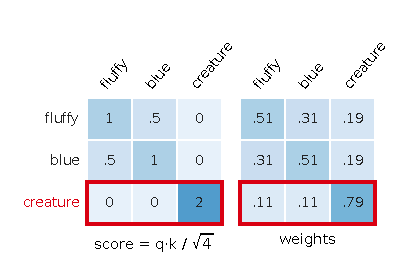
\includegraphics[width=\linewidth]{att_raw_grid.pdf}
  \end{columns}
  \vskip 4pt
  \trapbox{Raw vectors ask ``who is like me?'', and the answer is always ``me''. Creature wants
  its adjectives.}
\end{frame}

\milestone{\pQK}{Piece 1: $QK^\top$}{Who matches whom? Creature needs a better question than
``who is like me?''.}
\setpiece{\pQK}

\begin{frame}{A soft dictionary lookup}
  \begin{center}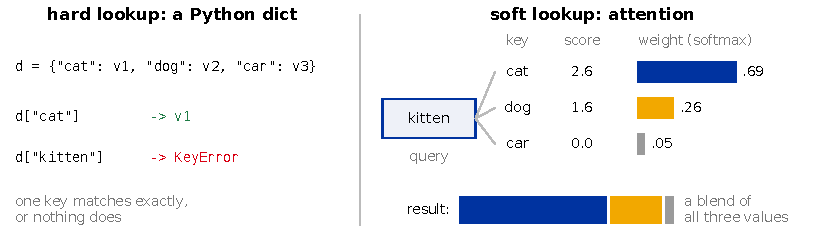
\includegraphics[width=0.92\linewidth]{att_soft_lookup.pdf}\end{center}
  \vskip -2pt
  {\small A \textbf{query} is what you want. A \textbf{key} is the label an entry is filed under.
  A \textbf{value} is what the entry contains.}
  \vskip 6pt
  \keybox{A dictionary is a \textbf{hard} lookup: one key matches exactly, or nothing does.
  Attention is a \textbf{soft} lookup: \emph{every} key matches a little, and you get a blend of
  all the values. Every word makes its own query, key and value, each with its own learned
  matrix. That is how creature can stop asking ``who is like me?''.}
\end{frame}

\begin{frame}{Query: ``what am I looking for?''}
  \begin{columns}[T]
    \column{0.55\textwidth}
    \begin{center}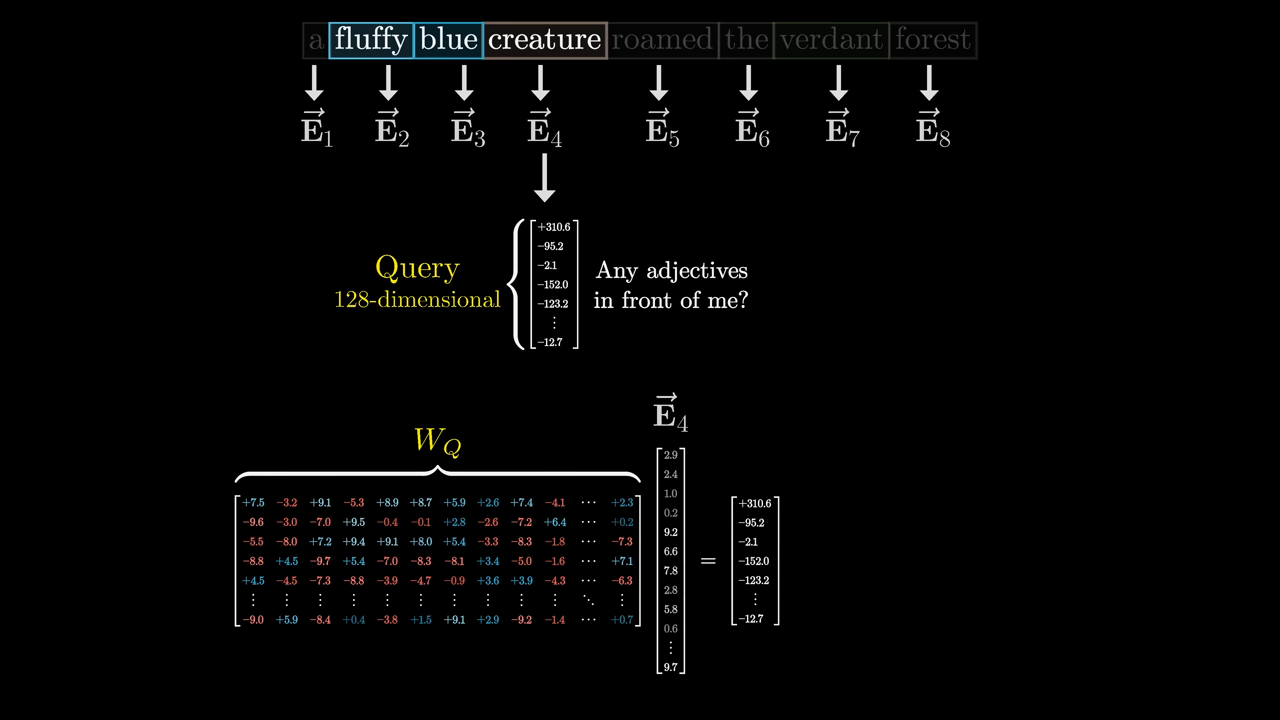
\includegraphics[width=\linewidth]{query_matrix.png}\end{center}
    \column{0.45\textwidth}
    Multiply a word's vector by a learned matrix $W_Q$ ($d_k \times d$, so $64 \times 768$; the
    \textbf{same} $W_Q$ for every word) to get its \textbf{query}, a shorter vector; its length is
    called $d_k$ (64 per head in GPT-2):
    \[ \mathbf{q}_i = W_Q\, \mathbf{e}_i . \]
    Creature's query can encode the question \emph{``any adjectives in front of me?''}
    \vskip 4pt
    \fcolorbox{popblue}{popblue!8}{\parbox{0.95\linewidth}{\scriptsize
      $W_Q$ is \textbf{learned}: nobody writes ``adjectives?'' into it. Backprop from the
      next-token loss adjusts it like any other weight; the questions that survive are the ones
      that help predict.}}
  \end{columns}
  \vskip 1pt {\scriptsize\color{gray} 3Blue1Brown (drawn for GPT-3: 128 numbers per query; GPT-2
  uses 64)}
\end{frame}

\begin{frame}{Key: ``what do I offer?''}
  \begin{columns}[T]
    \column{0.55\textwidth}
    \begin{center}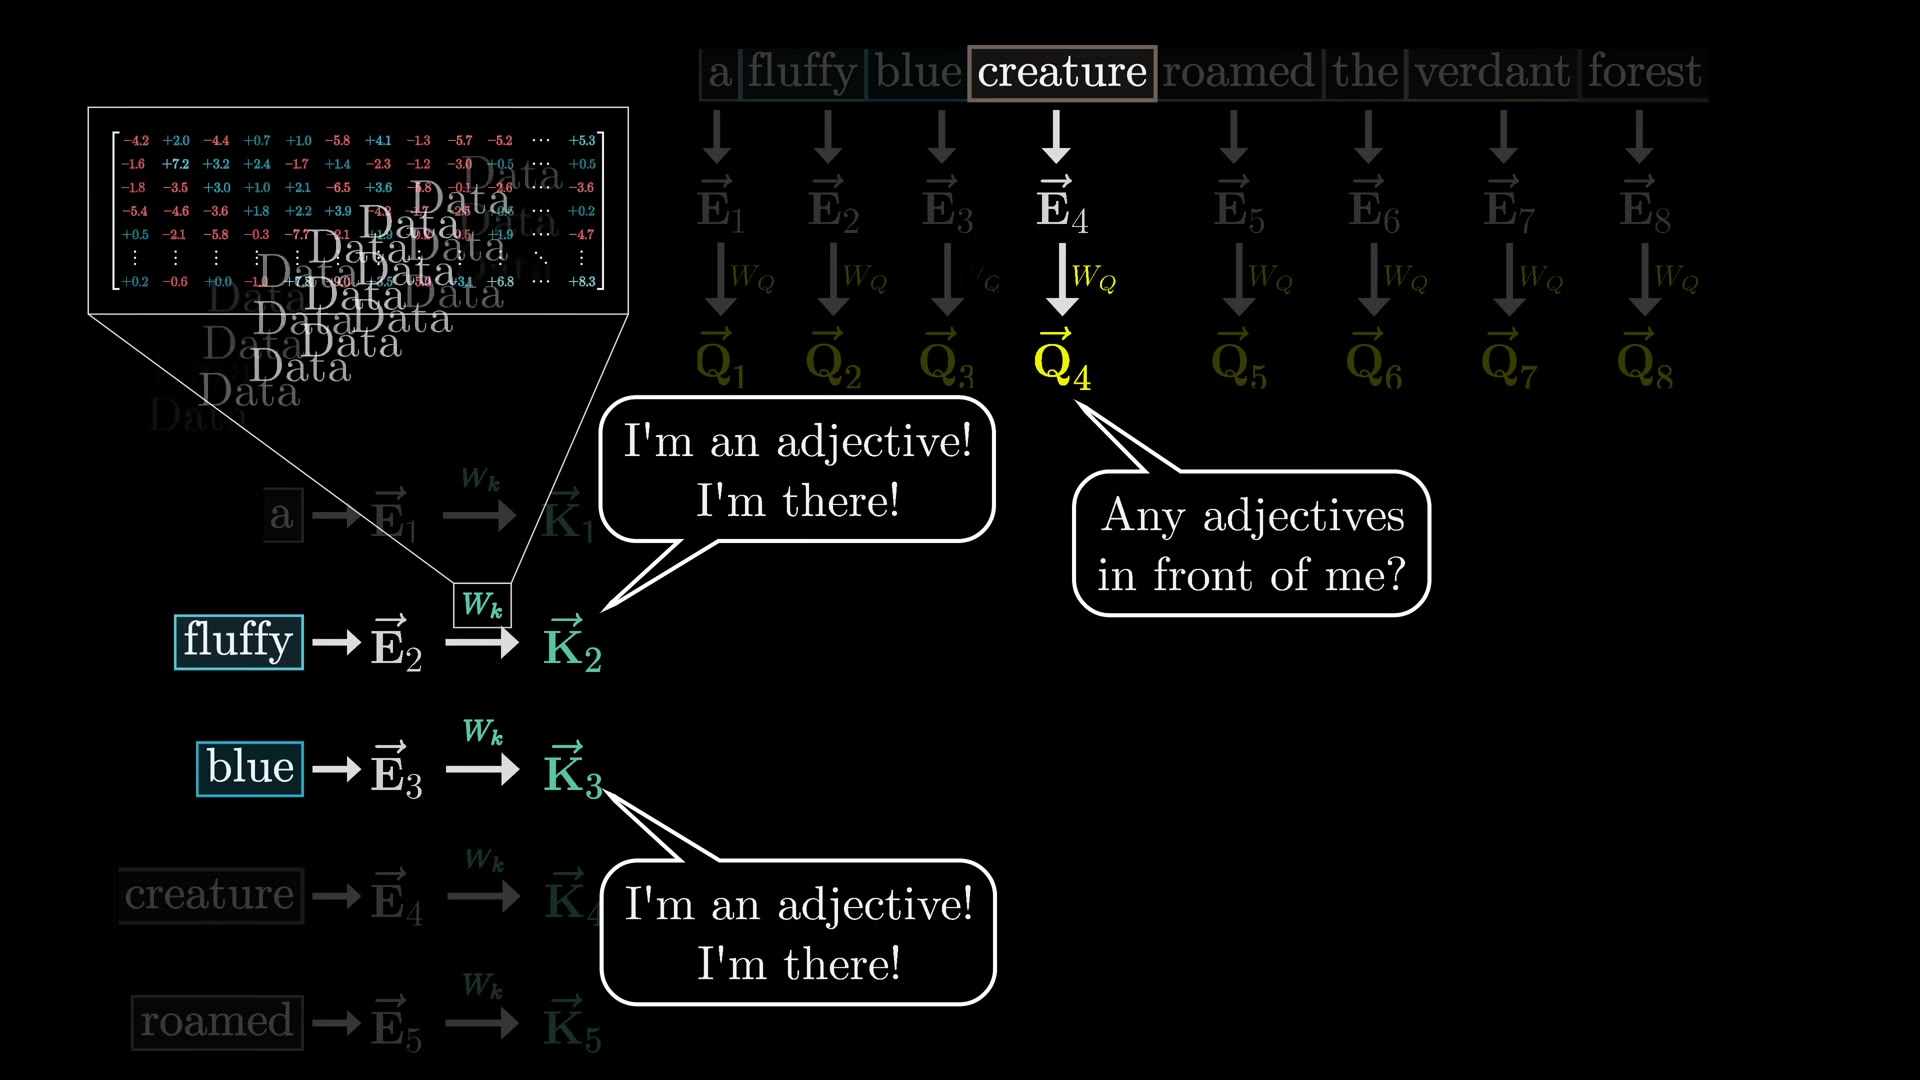
\includegraphics[width=\linewidth]{fs_key.jpg}\end{center}
    \column{0.45\textwidth}
    A second learned matrix $W_K$ turns each vector into a \textbf{key}:
    \[ \mathbf{k}_j = W_K\, \mathbf{e}_j . \]
    A key \emph{answers} queries. Fluffy's key can encode \emph{``I am an adjective, sitting
    right here.''}
    \vskip 4pt
    \fcolorbox{orange1}{orange1!10}{\parbox{0.95\linewidth}{\scriptsize
      A key is a word \emph{advertising} itself, so that the right queries can find it.}}
  \end{columns}
  \vskip 1pt \bbb
\end{frame}

\begin{frame}{Queries and keys meet in one space}
  \begin{columns}[T]
    \column{0.58\textwidth}
    \begin{center}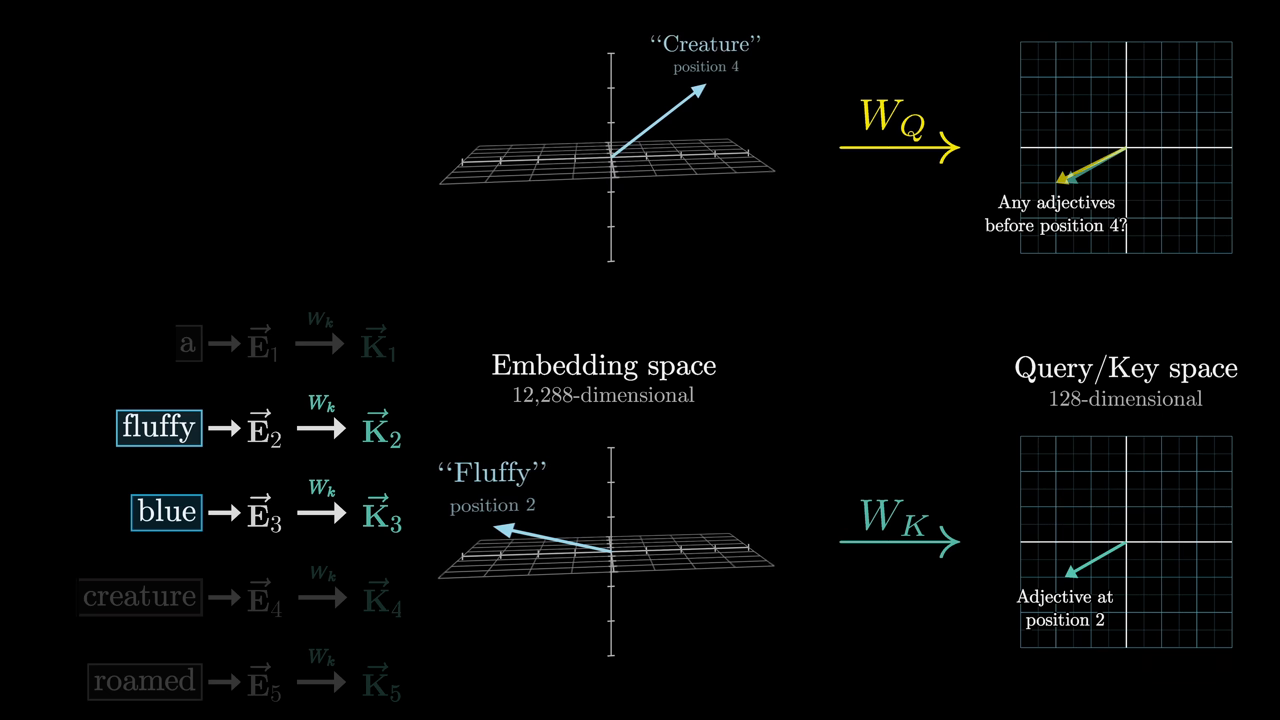
\includegraphics[width=\linewidth]{qk_space.png}\end{center}
    \column{0.42\textwidth}
    $W_Q$ and $W_K$ \textbf{project} the big embedding space down to a shared, smaller
    \textbf{query/key space} (project: multiply by a matrix that makes the vector shorter, 768
    numbers in, 64 out).
    \vskip 6pt
    Good $W_Q$, $W_K$ arrange it so that creature's query (``adjectives before me?'') and
    fluffy's key (``adjective, here'') point the \textbf{same way}.
    \vskip 6pt
    \fcolorbox{paramgreen}{paramgreen!8}{\parbox{0.95\linewidth}{\scriptsize
      That is all $W_Q$ and $W_K$ do: learn a space where ``relevant'' means ``pointing the same
      way''.}}
  \end{columns}
  \vskip 1pt \bbb
\end{frame}

\begin{frame}{The dot product scores relevance}
  \begin{columns}[T]
    \column{0.5\textwidth}
    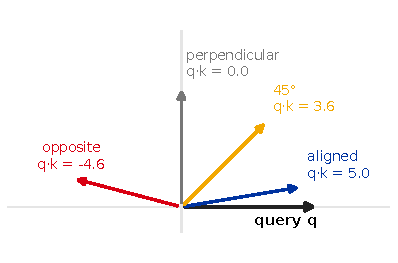
\includegraphics[width=\linewidth]{att_dot_product.pdf}
    \column{0.48\textwidth}
    $\mathbf{q}\cdot\mathbf{k}=|\mathbf{q}|\,|\mathbf{k}|\cos\theta$ is \textbf{large} when
    the two point the same way, \textbf{zero} when they are perpendicular, and
    \textbf{negative} when they point apart.
    \vskip 6pt
    So ``how relevant is this key to my query?'' collapses to \textbf{one number}.
    \vskip 6pt
    \keybox{All queries against all keys at once is one matrix product: $S = QK^\top$. Row $i$
    holds word $i$'s scores against every word.}
  \end{columns}
\end{frame}

\begin{frame}{By hand: ask a different question}
  \begin{columns}[T]
    \column{0.46\textwidth}
    \small
    Make the query/key space as small as it gets: \textbf{one} number, a single axis that means
    ``adjective match''. (GPT-2's heads use 64 numbers: room for 64 kinds of question.)
    \vskip 5pt
    \textcolor{popblue}{$w_Q = (0,0,0,1)$} reads the noun cell: a \textbf{noun} asks along that
    axis, ``any adjectives?''.
    \vskip 4pt
    \textcolor{orange1}{$w_K = (1,0,0,0)$} reads the adjective cell: an \textbf{adjective}
    answers on the same axis, ``adjective here''.
    \vskip 5pt
    Score = query $\times$ key, divided by $\sqrt{1} = 1$; then softmax by rows, as before.
    \column{0.52\textwidth}
    \vskip 2pt
    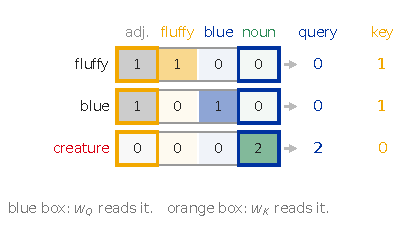
\includegraphics[width=\linewidth]{att_qk_axis.pdf}
  \end{columns}
  \vskip 8pt
  \keybox{\textbf{Predict:} what are creature's three weights now? And whom does fluffy listen
  to?}
\end{frame}

\begin{frame}{Creature finds its adjectives}
  \begin{columns}[T]
    \column{0.48\textwidth}
    \small
    Creature's scores: $2 \times 1,\ 2 \times 1,\ 2 \times 0 = 2,\ 2,\ 0$. Softmax:
    \[ \frac{(e^2,\ e^2,\ e^0)}{2e^2 + 1} = \frac{(7.39,\ 7.39,\ 1)}{15.78} \]
    \[ = (\mathbf{0.47},\ \mathbf{0.47},\ 0.06) \]
    Fluffy's query is $0$, so all its scores are $0$: it asks for nothing and spreads evenly,
    $0.33$ each.
    \vskip 4pt
    Each \textbf{row} sums to 1, a word's attention budget; the columns do not.
    \column{0.5\textwidth}
    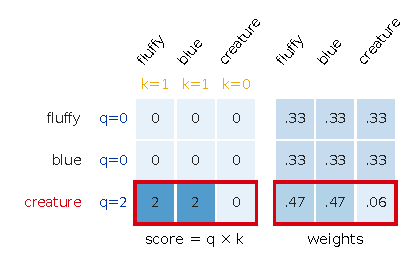
\includegraphics[width=\linewidth]{att_learned_grid.pdf}
  \end{columns}
  \vskip 4pt
  \takebox{Creature now asks ``any adjectives?'' (79\% on itself before, 6\% now). And the grid
  is no longer symmetric: creature $\to$ fluffy scores 2, fluffy $\to$ creature scores 0.}
\end{frame}

\milestone{\pSM}{Piece 2: softmax}{Scores can be any number, even negative. Weights must be
positive and add up to 1.}
\setpiece{\pSM}

\begin{frame}{Why softmax? 1: positive weights that sum to 1}
  \begin{columns}[T]
    \column{0.5\textwidth}
    Raw scores can be any real number. But we want a \textbf{weighted average} of the values, so
    the weights must be
    \begin{itemize}\small
      \item non-negative, and
      \item sum to $1$ (a distribution over ``where to look'').
    \end{itemize}
    \vskip 4pt
    Dividing by the sum fixes the second but not the first (middle): a negative score gives a
    negative weight. \textbf{Softmax} exponentiates first, so every weight is positive, then
    divides.
    \column{0.48\textwidth}
    \vskip 6pt
    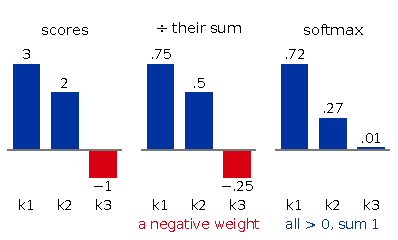
\includegraphics[width=\linewidth]{att_softmax_why.pdf}
  \end{columns}
  \vskip 10pt
  \keybox{$\mathrm{softmax}(s)_j = e^{s_j} / \sum_i e^{s_i}$: positive because $e^{x} > 0$ for
  every $x$, and the division makes the weights sum to 1.}
\end{frame}

\begin{frame}{Why softmax? 2: soft, so it can learn}
  \begin{columns}[T]
    \column{0.5\textwidth}
    \small
    Why not just pick the best key (argmax)? Slide one key's score and watch its weight.
    \vskip 5pt
    \textcolor{armred}{\textbf{argmax}} jumps from 0 to 1 the moment the key takes the lead, and
    is flat everywhere else. A small change of the score changes nothing, so the gradient is 0
    and backprop gets no signal.
    \vskip 5pt
    \textcolor{popblue}{\textbf{softmax}} moves a little for every little change: a slope
    everywhere, so training can push the weights where they need to go. And it spreads weight
    over all the good keys instead of picking one.
    \column{0.48\textwidth}
    \vskip 2pt
    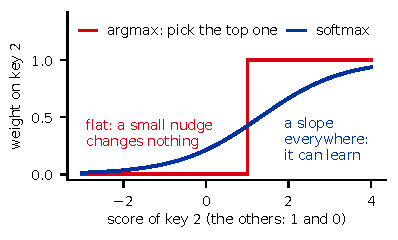
\includegraphics[width=\linewidth]{att_argmax_softmax.pdf}
  \end{columns}
  \vskip 8pt
  \watchbox{One catch: the weights must sum to 1, so a head can never look at \emph{nothing}.
  LLM-4 shows where real heads park the weight they do not need (attention sinks).}
\end{frame}

\milestone{\pSQ}{Piece 3: $\sqrt{d_k}$}{Why divide by this one number? \textbf{Predict:} do
scores from 64-number vectors come out bigger or smaller than from 4-number ones?}
\setpiece{\pSQ}

\begin{frame}{More numbers, bigger scores}
  \begin{center}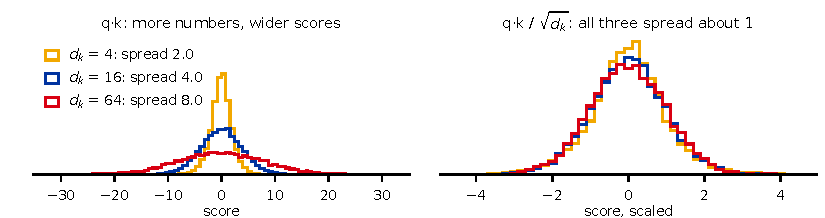
\includegraphics[width=\linewidth]{att_dk_spread.pdf}\end{center}
  \vskip -4pt
  {\small A dot product over $d_k$ numbers is a sum of $d_k$ products. If the numbers have spread
  1, each product has variance 1, and variances add: the sum has variance $d_k$, spread
  $\sqrt{d_k}$. Measured on 10{,}000 random pairs each: about 2, 4 and 8 (8.05 for $d_k = 64$).}
  \vskip 6pt
  \keybox{Bigger. GPT-2's heads use $d_k = 64$, so raw scores swing by about $\pm 8$, not $\pm 1$.
  Right: divide by $\sqrt{d_k}$ and all three are back to spread 1.}
\end{frame}

\begin{frame}{Big scores freeze softmax}
  \begin{columns}[T]
    \column{0.5\textwidth}
    \small
    The same three keys, with the winner's lead growing: $(1,0,0)$, $(2,0,0)$, $(4,0,0)$,
    $(8,0,0)$. Softmax goes from a soft preference to one weight near 1: it
    \textbf{saturates}.
    \vskip 5pt
    Now nudge a loser up by 1. At $(8, 0, 0)$ its weight goes from 0.0003 to 0.0009. At
    $(1, 0, 0)$ the same nudge moves it from 0.21 to 0.42.
    \vskip 5pt
    A nudge that changes nothing gives the gradient nothing to work with: \textbf{training
    stalls}. It is argmax's flat part all over again.
    \column{0.48\textwidth}
    \vskip 4pt
    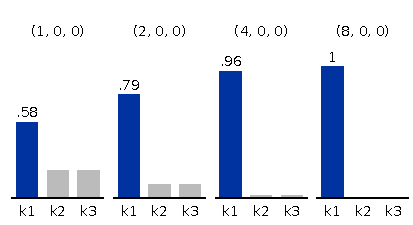
\includegraphics[width=\linewidth]{att_saturation.pdf}
  \end{columns}
\end{frame}

\begin{frame}{The fix: divide by $\sqrt{d_k}$}
  \begin{columns}[T]
    \column{0.5\textwidth}
    \small
    Divide every score by the spread, $\sqrt{d_k} = 8$: the scores are back to about $\pm 1$,
    softmax stays soft, and every key keeps a slope.
    \vskip 5pt
    Right: five random keys, $d_k = 64$. Raw, one key takes everything. Divided by 8, all five
    keep a share.
    \vskip 6pt
    \fcolorbox{warnred}{warnred!8}{\parbox{0.95\linewidth}{\scriptsize
      Why not divide by $d_k = 64$? That would squash the scores near 0, and softmax would go
      flat: every key about the same weight, however relevant. $\sqrt{d_k}$ is the number that
      makes the spread exactly 1.}}
    \column{0.5\textwidth}
    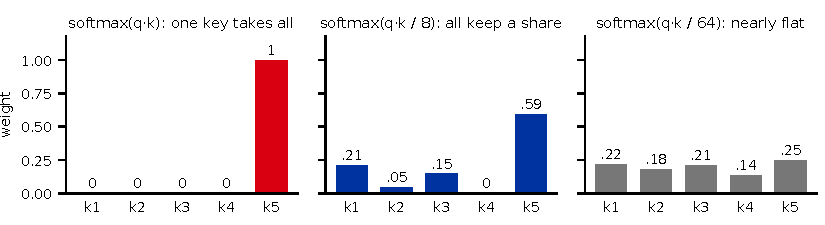
\includegraphics[width=\linewidth]{att_sqrt_dk.pdf}\\
    {\scriptsize Five random keys, $d_k = 64$: the same scores, before and after dividing by 8.}
  \end{columns}
  \vskip 6pt
  {\scriptsize\color{gray} Karpathy shows the same effect in code at 1:16:56 of ``Let's build
  GPT'' (link on the first slide).}
\end{frame}

\milestone{\pV}{Piece 4: $V$}{The weights say whom to listen to. What do those words actually
say?}
\setpiece{\pV}

\begin{frame}{Value: ``what do I hand over?''}
  \begin{columns}[T]
    \column{0.55\textwidth}
    \begin{center}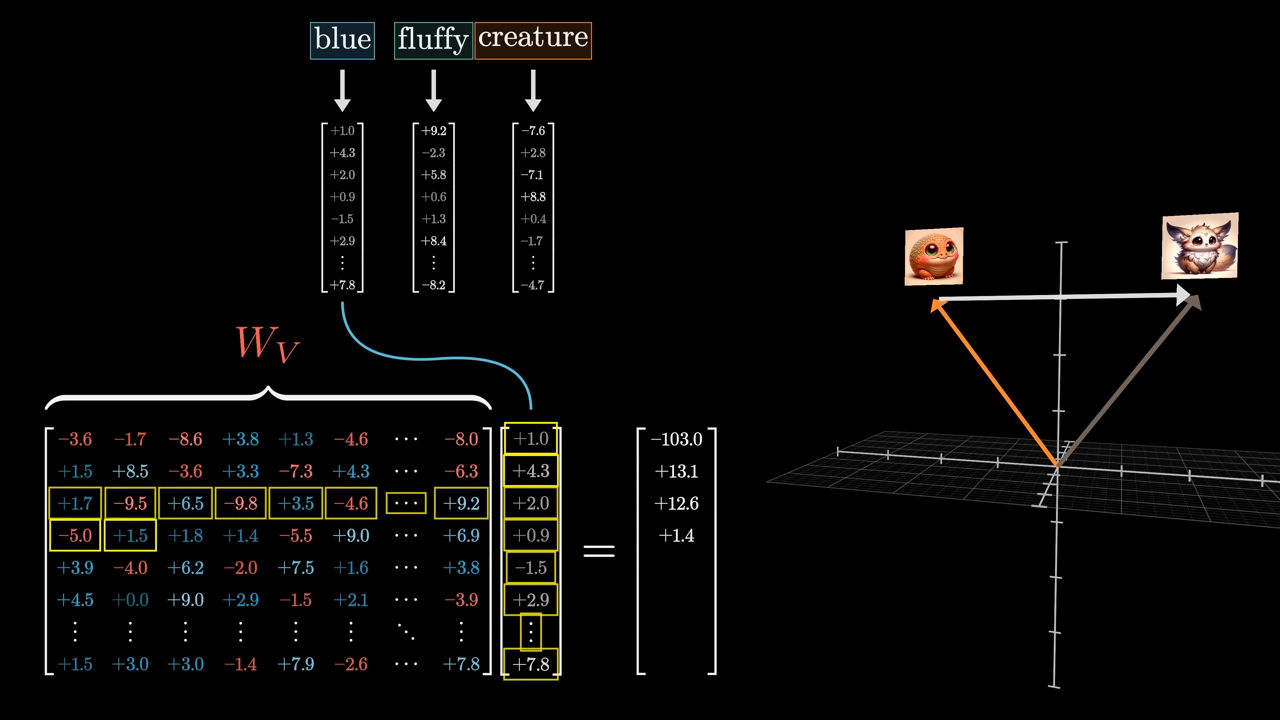
\includegraphics[width=\linewidth]{value_wv.png}\end{center}
    \column{0.45\textwidth}
    A third learned matrix $W_V$ makes each word's \textbf{value}, the information it hands
    over when attended to:
    \[ \mathbf{v}_j = W_V\, \mathbf{e}_j . \]
    Fluffy's value is, roughly, ``the fluffiness to add to a noun''.
    \vskip 4pt
    \fcolorbox{paramgreen}{paramgreen!10}{\parbox{0.95\linewidth}{\scriptsize
      Key $=$ how you are \emph{found}; value $=$ what you \emph{give}. Different jobs, different
      matrices.}}
  \end{columns}
  \vskip 1pt \bbb
\end{frame}

\begin{frame}{By hand: what gets handed over}
  \begin{center}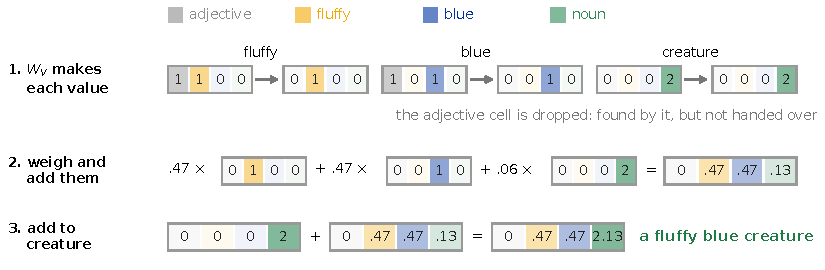
\includegraphics[width=0.92\linewidth]{att_value_chips.pdf}\end{center}
  \vskip -4pt
  {\small Creature's weights 0.47, 0.47, 0.06 come from piece 1 (0.468 and 0.063 to three
  digits, so $0.063 \times 2 = 0.13$). Step 3 is the residual connection (LLM-4). With raw
  vectors the result was $(0.21,\ 0.11,\ 0.11,\ 3.57)$: mostly more creature.}
  \vskip 5pt
  \takebox{Fluffy was \emph{found} by its label (``adjective'') and \emph{handed over} its
  content (fluffiness). Found by one thing, give another: that is why $W_K \neq W_V$.}
\end{frame}

\begin{frame}{The output: values, weighted and summed}
  \begin{columns}[T]
    \column{0.5\textwidth}
    \begin{center}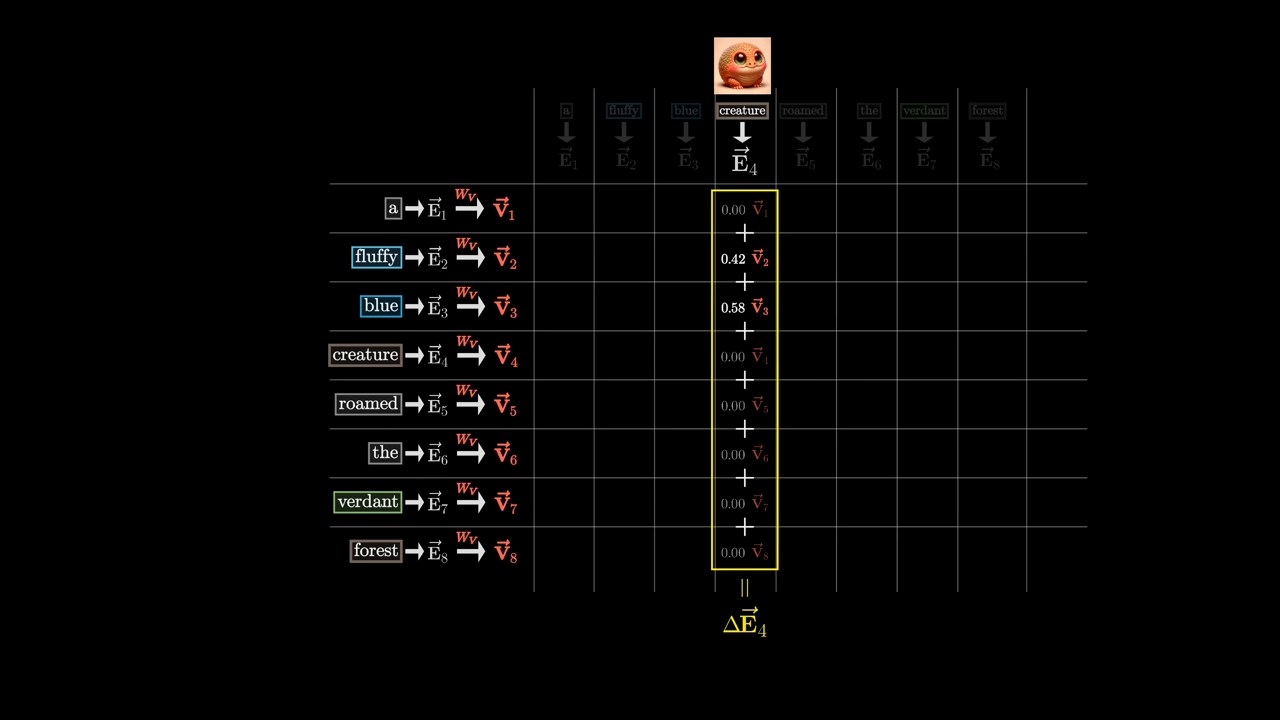
\includegraphics[width=\linewidth]{value_delta_e.png}\end{center}
    \column{0.5\textwidth}
    In general: the weights say \emph{how much} to listen, the values say \emph{what} to pass.
    Word $i$'s output is
    \[ \mathbf{o}_i = \sum_j \alpha_{ij}\, \mathbf{v}_j \]
    \vskip -4pt
    {\small ($\alpha_{ij}$: the weight word $i$ gives word $j$.)}
    \vskip 4pt
    \fcolorbox{paramgreen}{paramgreen!8}{\parbox{0.95\linewidth}{\scriptsize
      Every word is updated this way \textbf{at once}, in one parallel step. The output is
      \textbf{added} to the word's own vector, so words \emph{refine} rather than overwrite
      (the residual connection; LLM-4's $W^O$ first maps a head's 64 numbers back to 768).}}
  \end{columns}
  \vskip 1pt \bbb
\end{frame}

\begin{frame}{Why three matrices?}
  One word plays \textbf{three roles} at once:
  \vskip 6pt
  \begin{center}\small
    \begin{tabular}{l l l}
      \textcolor{popblue}{\textbf{Query}} $\mathbf{q}=W_Q\mathbf{e}$ & what I am \emph{looking for}
        & creature: ``any adjectives?'' \\[3pt]
      \textcolor{orange1}{\textbf{Key}} $\mathbf{k}=W_K\mathbf{e}$ & how I am \emph{found}
        & fluffy: ``adjective, here'' \\[3pt]
      \textcolor{paramgreen}{\textbf{Value}} $\mathbf{v}=W_V\mathbf{e}$ & what I \emph{hand over}
        & fluffy: fluffiness, not the label \\
    \end{tabular}
  \end{center}
  \vskip 8pt
  \keybox{Without them, every word asks ``who is like me?'' and finds itself (79\% in our toy),
  and A and B score each other exactly the same. With them, the question, the label and the message are
  three separate things the model learns. They are the only weights in a single head (LLM-4 adds
  $W^O$ when heads are combined).}
\end{frame}

\milestone{\pALL}{The whole line}{Every piece has a job now. Read it once more, left to right.}
\setpiece{\pALL}

% the destination frame again, with every question answered
\begin{frame}{Putting it together: every piece has a job}
  \vskip 30pt
  \begin{center}
  {\LARGE $\displaystyle\mathrm{Attention}(Q,K,V) =
    \tikzmarknode{psm}{\textcolor{armred}{\mathrm{softmax}}}\!\Big(\frac{\tikzmarknode{pqk}{%
    \textcolor{popblue}{Q}\textcolor{orange1}{K^{\top}}}}{\tikzmarknode{psq}{\textcolor{violet1}{%
    \sqrt{d_k}}}}\Big)\,\tikzmarknode{pv}{\textcolor{paramgreen}{V}}$}
  \end{center}
  \begin{tikzpicture}[remember picture, overlay, font=\footnotesize, >=Latex]
    \node[text=popblue, align=center] (a) at ([shift={(1.3cm,1.2cm)}]pqk.north)
      {every query $\cdot$ every key:\\the $n \times n$ grid of scores};
    \draw[->, popblue, thick] (a.south) -- (pqk.north);
    \node[text=armred, align=center] (b) at ([shift={(-1.2cm,1.2cm)}]psm.north)
      {scores $\to$ weights,\\row by row};
    \draw[->, armred, thick] (b.south) -- (psm.north);
    \node[text=violet1, align=center] (c) at ([shift={(-2.9cm,-1.0cm)}]psq.south)
      {keeps the scores near $\pm 1$,\\so softmax stays soft};
    \draw[->, violet1, thick] (c.east) -- (psq.south west);
    \node[text=paramgreen, align=center] (d) at ([shift={(0.6cm,-1.0cm)}]pv.south)
      {what each word hands over,\\blended by the weights};
    \draw[->, paramgreen, thick] (d.north) -- (pv.south);
  \end{tikzpicture}
  \vskip 56pt
  \takebox{``Score, softmax, weighted sum'': the same three moves as wall 1, now with learned
  $Q$, $K$, $V$ from one sentence. In wall 1 the queries came from the decoder and the keys and
  values from the encoder: that version is \textbf{cross-attention} (LLM-5).}
\end{frame}

\begin{frame}{Shapes, on a real sentence}
  \begin{center}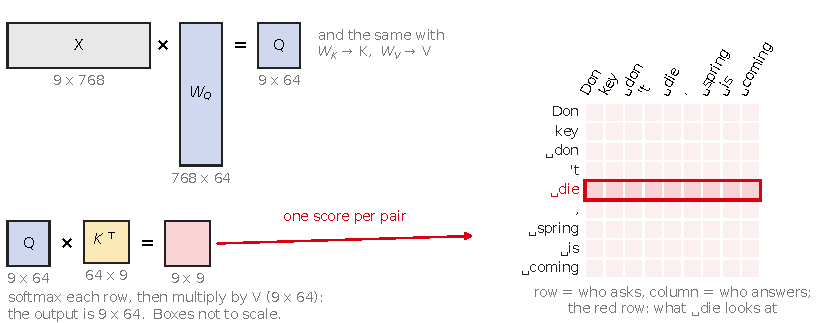
\includegraphics[width=\linewidth]{att_shapes.pdf}\end{center}
  \vskip -2pt
  {\small ``Donkey don't die, spring is coming'' is 6 words but 9 GPT-2 tokens (LLM-1): $n$
  counts tokens. The sizes 768 and 64 are GPT-2's.}
\end{frame}

\begin{frame}{The same shapes in GPT-2}
  \begin{center}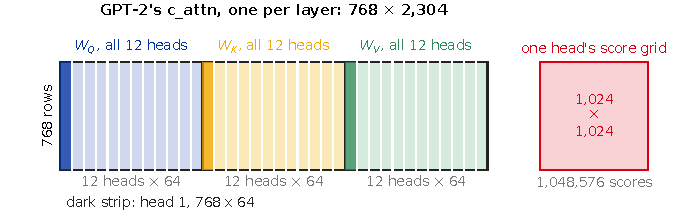
\includegraphics[width=0.84\linewidth]{att_gpt2_cattn.pdf}\end{center}
  \vskip -8pt
  {\small One head's $W_Q$, $W_K$, $W_V$ are $64 \times 768$ each in our $W_Q\,\mathbf{e}$
  notation; the file stores them \textbf{transposed}, all twelve heads' side by side, because
  code multiplies rows (next slide). Why 64 and not 768?
  $12 \times 64 = 768$: each head gets its own small space for its own question (LLM-4).}
  \vskip 3pt
  \watchbox{A full 1{,}024-token window: 150{,}994{,}944 scores over 12 heads and 12 layers.
  Double the text and the grid grows \textbf{four times}; $X$, $Q$, $K$, $V$ only double (LLM-5
  adds up the bill). \src{(GPT-2's config and weight file, 2026-10-05.)}}
\end{frame}

\begin{frame}[fragile]{Attention in about 10 lines}
  Every step is a matrix operation. In NumPy, with one token per \textbf{row} of \texttt{X}, so
  $\mathbf{q} = W_Q\,\mathbf{e}$ becomes \texttt{X @ Wq} with \texttt{Wq} $= W_Q^\top$
  ($768 \times 64$):
\begin{lstlisting}
import numpy as np

def attention(X, Wq, Wk, Wv):
    Q, K, V = X @ Wq, X @ Wk, X @ Wv       # three learned views
    d_k = Q.shape[1]
    scores = Q @ K.T / np.sqrt(d_k)         # relevance, scaled
    scores -= scores.max(1, keepdims=True)  # safe exp, same softmax
    weights = np.exp(scores)
    weights /= weights.sum(1, keepdims=True)  # softmax over each row
    return weights @ V                      # weighted sum of values
\end{lstlisting}
  \vskip 2pt
  \keybox{No loops over positions, no recurrence: three matrix products and a softmax. That
  simplicity is the whole point. Subtracting each row's max changes no weight (softmax only sees
  differences, LLM-5) and keeps \texttt{exp} from overflowing.}
\end{frame}

% ================================================================
% MASKING (2026-10-28; the causal mask frames moved here from LLM-4, py_src/masking_figs.py)
\section{Masking: who may look at whom}
\setpiece{}
\sectiontransition{Masking}{Who may look at whom? Two ways to learn from raw text.}

\begin{frame}{Two fill-in games}
  A model learns from raw text by playing a fill-in game: hide a word, guess it, compare with
  the truth. No labels needed. Two versions on our sentence:
  \vskip 6pt
  \begin{center}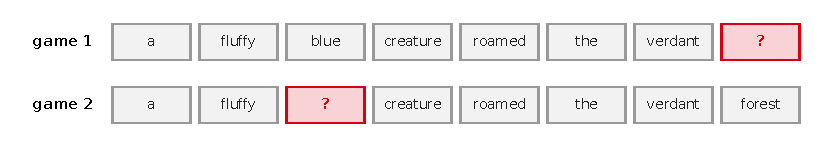
\includegraphics[width=\linewidth]{mask_two_games.pdf}\end{center}
  \vskip 6pt
  \keybox{\textbf{Predict:} which words may the model use to fill each blank? And which game
  teaches a model to \emph{write}, one word after another?}
\end{frame}

\begin{frame}{Game 1: causal language modeling}
  \begin{center}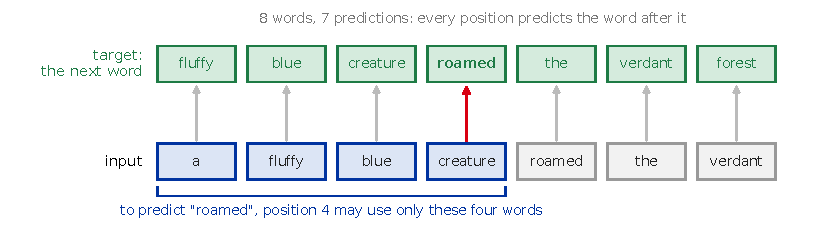
\includegraphics[width=\linewidth]{mask_clm_shift.pdf}\end{center}
  \vskip -2pt
  {\small Shift the sentence by one: the target at every position is the next word. Each
  position may use only the words up to itself: the past can cause the next word, the future
  cannot. Hence the name \textbf{causal language modeling} (CLM), also called next-token
  prediction or \emph{autoregressive} modeling.}
  \vskip 6pt
  \takebox{This is GPT's game \paper{(Radford et al., 2018)}, and what GPT-2 was trained on.
  Writing is the same game for real: predict a word, append it, predict again (LLM-5, LLM-6).}
\end{frame}

\begin{frame}{The cheat}
  \begin{columns}[T]
    \column{0.5\textwidth}
    \small
    Self-attention lets every word look at every word. Train game 1 like that, and ``blue'',
    which must predict ``creature'', can simply \textbf{look at} ``creature'': it is the next
    word in the input.
    \vskip 5pt
    One head learns ``copy the word to my right'', and the training loss falls towards 0.
    \vskip 5pt
    Then you ask it to write. The next word does not exist yet, there is nothing to copy, and
    the model has learned nothing it can use.
    \column{0.48\textwidth}
    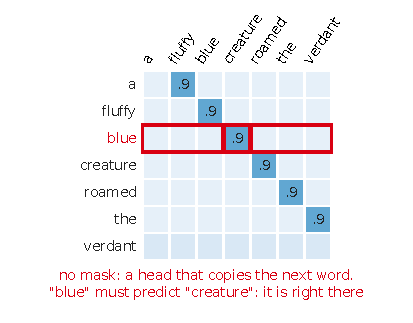
\includegraphics[width=\linewidth]{mask_cheat.pdf}
  \end{columns}
  \vskip 4pt
  \trapbox{Whatever a position looks at in training must also exist when the model writes. So:
  forbid every position to look to its right.}
\end{frame}

\bbbcap{fs_masking.jpg}{The fix has a name: \emph{masking}. Before the softmax, every entry above
the diagonal is set to $-\infty$, so after it each word sees only itself and the words before.}

\begin{frame}{The mask in three steps}
  \begin{center}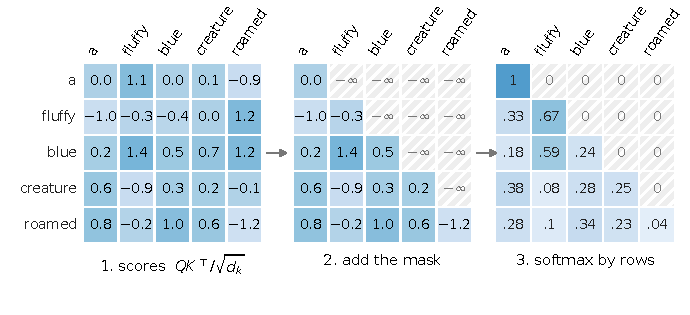
\includegraphics[width=0.8\linewidth]{mask_steps.pdf}\end{center}
  \vskip -6pt
  {\small Add a matrix $M$ to the scores \emph{before} the softmax: $0$ on and below the
  diagonal, $-\infty$ above it. $e^{-\infty} = 0$, so every future word gets weight
  \textbf{exactly} 0, and each row still sums to 1.}
  \vskip 4pt
  \keybox{$\mathrm{softmax}\big(QK^\top/\sqrt{d_k} + M\big)\,V$: the same line plus one fixed
  matrix. No new weights, nothing to learn.}
\end{frame}

\begin{frame}{By hand: the mask on creature's grid}
  \begin{columns}[T]
    \column{0.46\textwidth}
    \small
    The learned grid from piece 1 (queries ask ``any adjectives?'', keys answer ``adjective
    here''), now with the mask:
    \begin{itemize}
      \item \textbf{fluffy} (red) sees only itself: $(0.33, 0.33, 0.33) \to (1, 0, 0)$;
      \item blue sees fluffy and itself, scores $0, 0$: $(0.5, 0.5, 0)$;
      \item creature's row does not change: $(0.47, 0.47, 0.06)$.
    \end{itemize}
    \column{0.52\textwidth}
    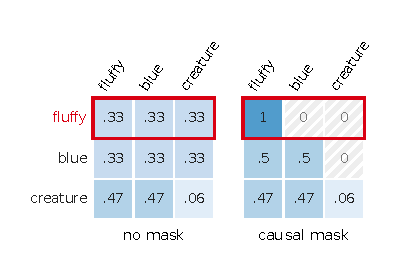
\includegraphics[width=\linewidth]{mask_creature_grid.pdf}
  \end{columns}
  \vskip 6pt
  \takebox{In English adjectives come before their noun, so a left-to-right model can still let
  the noun gather them. What the mask removes is the other direction.}
\end{frame}

\begin{frame}{Why $-\infty$ before the softmax, and not 0 after?}
  \begin{columns}[T]
    \column{0.5\textwidth}
    \small
    Row ``fluffy'' of the three-step grid: scores $-1.0$ and $-0.3$ for a and fluffy, then
    $-0.4$, $0.0$ and $1.2$ for the three words after it.
    \vskip 5pt
    \textbf{Zero after:} softmax over all five hands the future 82\% of the weight (``roamed''
    alone 0.54). Zero those and what is left, $0.06 + 0.12$, sums to 0.18: no longer a weighted
    average.
    \vskip 5pt
    \textbf{$-\infty$ before:} the softmax only ever sees a and fluffy: $0.33$ and $0.67$. The
    same 1 to 2 ratio, now summing to 1.
    \column{0.48\textwidth}
    \vskip 4pt
    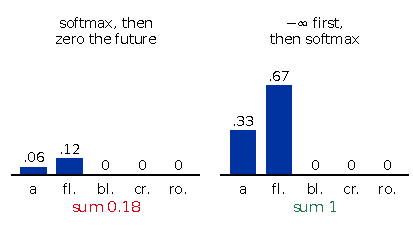
\includegraphics[width=\linewidth]{mask_renorm.pdf}
  \end{columns}
  \vskip 6pt
  \keybox{Masking is a softmax over the visible keys only. (Zeroing after and dividing by 0.18
  gives the same answer; adding $-\infty$ does it in one step.)}
\end{frame}

\begin{frame}{One pass, every prefix at once}
  \begin{center}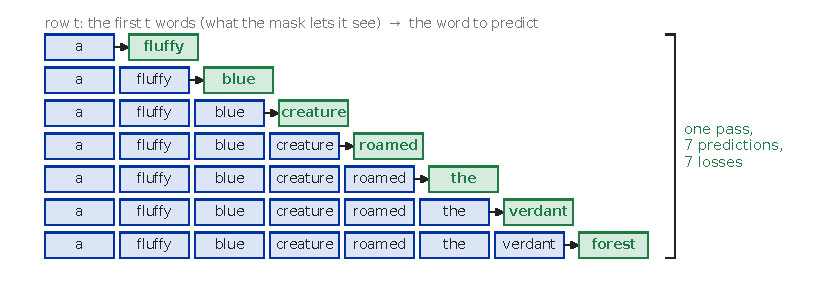
\includegraphics[width=0.86\linewidth]{mask_one_pass.pdf}\end{center}
  \vskip -6pt
  {\small Without the mask, each prediction needs its own pass with the future cut off: feed the
  first $t$ words, predict word $t{+}1$, seven times. With the mask, row $t$ of the grid
  \emph{is} that cut: one pass over 8 words gives \textbf{7 training signals}, none can cheat.}
  \vskip 4pt
  \keybox{A large part of why pretraining on internet-scale text is affordable at all. The causal
  mask is not a safety measure; it is a \textbf{throughput} decision that happens to enforce
  correctness (LLM-7 comes back to it).}
\end{frame}

\begin{frame}{Game 2: masked language modeling}
  \begin{center}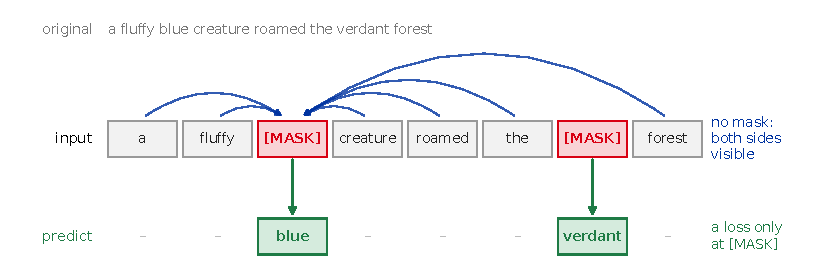
\includegraphics[width=0.94\linewidth]{mask_mlm.pdf}\end{center}
  \vskip -6pt
  {\small Hide some words by replacing them with a special token, \texttt{[MASK]}, and predict
  the originals. There is \textbf{no attention mask}: every word, \texttt{[MASK]} included, sees
  both sides. This is \textbf{masked language modeling} (MLM), BERT's game
  \paper{(Devlin et al., 2019)}: about 15\% of the tokens are hidden (here 2 of 8), and only those
  give a loss.}
  \vskip 4pt
  \takebox{The predict's answer: game 1 may use only the words before the blank, game 2 the words
  on both sides, and only game 1 can write. BERT's exact recipe is in LLM-7.}
\end{frame}

\begin{frame}{CLM vs MLM}
  \begin{center}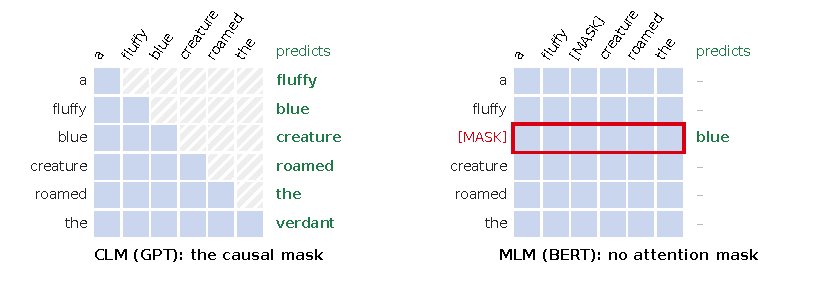
\includegraphics[width=0.94\linewidth]{mask_clm_vs_mlm.pdf}\end{center}
  \vskip -6pt
  \begin{center}\small
  \begin{tabular}{lll}
    \toprule
    & \textbf{CLM} (GPT) & \textbf{MLM} (BERT) \\
    \midrule
    who may look & the past only & everyone, both sides \\
    a loss at & every position: $n$ per pass & the hidden ones: about $0.15\,n$ \\
    can it write? & yes, one word at a time & no: it needs the words on both sides \\
    \bottomrule
  \end{tabular}
  \end{center}
\end{frame}

\begin{frame}{Two different things called ``mask''}
  \begin{center}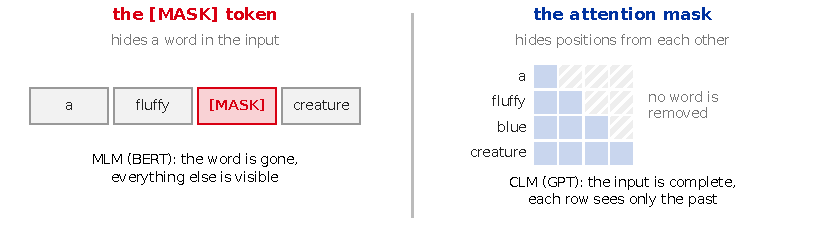
\includegraphics[width=\linewidth]{mask_two_kinds.pdf}\end{center}
  \vskip 6pt
  \trapbox{\texttt{[MASK]} is a \textbf{token}: it changes the input, and the model sees
  everything else (MLM, BERT). The \textbf{attention mask} is a matrix added to the scores: the
  input is complete, but each position may look only at some of the others (CLM, GPT). One word,
  two different mechanisms.}
\end{frame}

\begin{frame}{One more mask: padding}
  \begin{center}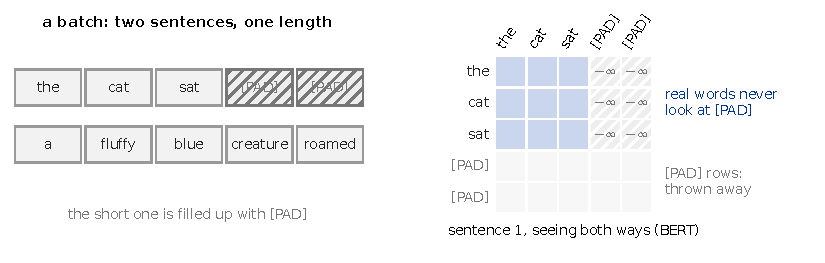
\includegraphics[width=0.94\linewidth]{mask_padding.pdf}\end{center}
  \vskip -6pt
  {\small A GPU wants a batch to be one rectangle, so shorter sentences are filled up with a
  \texttt{[PAD]} token. Nobody should read it: its columns get $-\infty$ too (the same trick), and
  the outputs at the \texttt{[PAD]} rows are thrown away.}
  \vskip 4pt
  \watchbox{With a causal mask and the padding at the end, real words never see it anyway. It
  matters when the model sees both ways (BERT), and when a batch of prompts is padded at the
  front for writing. Pretraining usually packs documents end to end and needs no padding (LLM-7).}
\end{frame}

% ================================================================
\section*{Recap}

\begin{frame}{One head, end to end}
  \begin{columns}[T]
    \column{0.52\textwidth}
    \begin{center}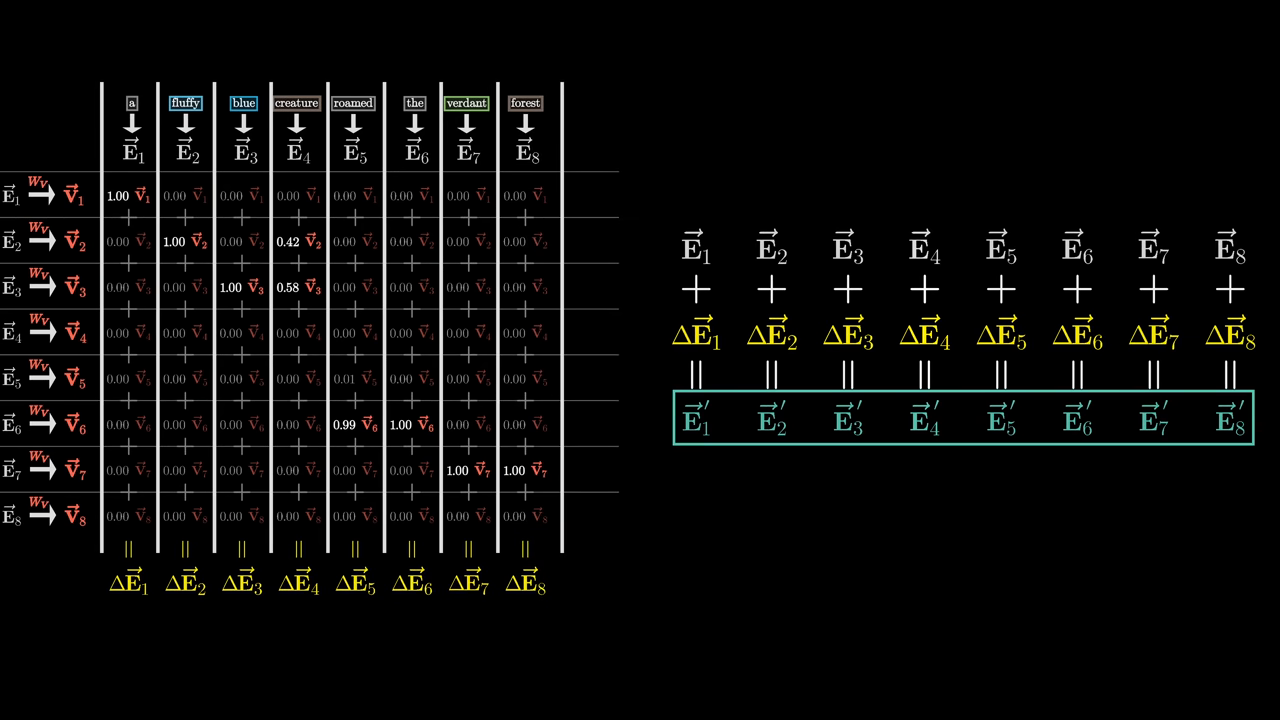
\includegraphics[width=\linewidth]{single_head_full.png}\end{center}
    \bbb
    \column{0.46\textwidth}
    \begin{itemize}\small
      \item \textbf{Wall 1}, one $C$: every step gets its own weighted mix of the inputs.
      \item \textbf{Wall 2}, the queue: self-attention builds every vector at once.
      \item Each word makes a \textcolor{popblue}{query}, a \textcolor{orange1}{key} and a
        \textcolor{paramgreen}{value}: ask, get found, hand over. Without them a word listens
        to itself.
      \item Score $QK^\top/\sqrt{d_k}$, softmax by rows, weighted sum of values; the grid is
        $n \times n$.
      \item The \textbf{causal mask} keeps CLM (GPT) from peeking; MLM (BERT) hides words and
        sees both sides.
    \end{itemize}
    \takebox{\textbf{Next (LLM-4):} many heads at once, and the block around them.}
  \end{columns}
\end{frame}

\begin{frame}{Try it yourself}
  \vskip 8pt
  Back to the demo from the first slide:
  \href{https://poloclub.github.io/transformer-explainer/}{\textbf{Transformer Explainer}}
  (\texttt{poloclub.github.io/transformer-explainer}) runs GPT-2 small in your browser. Type
  your own sentence and look at the attention weights: the same $QK^\top$, softmax and $\times V$
  as today, on a real model.
  \vskip 12pt
  \keybox{Real heads are messier than the creature toy, and different heads do different jobs.
  That is where LLM-4 starts.}
\end{frame}

\begin{frame}{Careful: attention weights are not explanations}
  \begin{itemize}
    \item The grids are tempting: ``the model looked at fluffy, so that is why it answered''.
      Jain \& Wallace (NAACL 2019) tested it: attention weights often disagree with other measures
      of which inputs matter, and very different weights can give the same prediction. Their
      title: ``Attention is not Explanation''.
    \item Wiegreffe \& Pinter (EMNLP 2019) answered with ``Attention is not \emph{not}
      Explanation'': it depends on what you call an explanation, and the swapped-in weights fail
      closer tests.
    \item Both studied RNNs with attention, not GPT. The lesson carries over: a weight shows where
      one head looked, not why the model answered.
  \end{itemize}
  \vskip 6pt
  \keybox{Use the demo to see \emph{what} heads do. Testing \emph{why} takes interventions:
  change something inside the model and watch the answer (LLM-4 has one; the interpretability
  chapter has many).}
\end{frame}

\begin{frame}{Next on the map}
  \begin{center}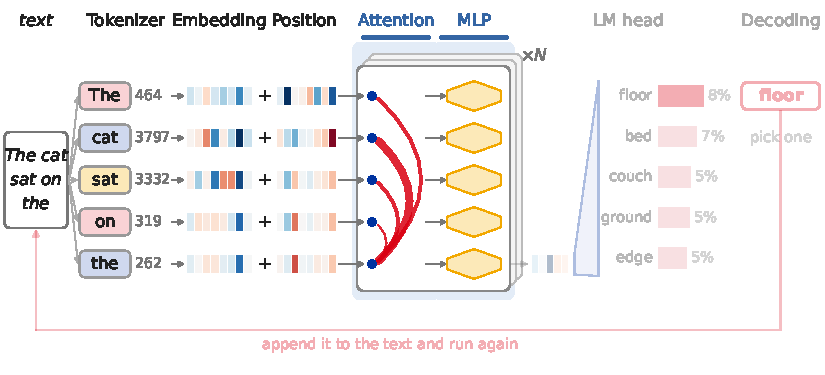
\includegraphics[width=\linewidth]{roadmap_block_pass.pdf}\end{center}
  \vskip -2pt
  {\small Next (LLM-4): many heads at once, and the block around them.}
\end{frame}

\begin{frame}{Sources \& further reading}
  \footnotesize
  \begin{itemize}
    \item Bahdanau, Cho \& Bengio (2015), \emph{Neural Machine Translation by Jointly Learning to
      Align and Translate}: attention, for translation.
    \item Xu et al.\ (2015), \emph{Show, Attend and Tell}: attention for image captioning.
    \item Vaswani et al.\ (2017), \emph{Attention Is All You Need}: self-attention, the
      Transformer.
    \item Radford et al.\ (2018), \emph{Improving Language Understanding by Generative
      Pre-Training} (GPT, causal LM); Devlin et al.\ (2019), \emph{BERT} (masked LM), NAACL.
    \item Jay Alammar, \emph{The Illustrated Transformer}; Andrej Karpathy (2023),
      \link{https://youtu.be/kCc8FmEb1nY?t=2533}{Let's build GPT: from scratch, in code, spelled
      out.}
    \item Jain \& Wallace (2019), ``Attention is not Explanation'', NAACL; Wiegreffe \& Pinter
      (2019), ``Attention is not not Explanation'', EMNLP. Levy (2024), Wired, on the paper's
      history.
    \item Transformer Explainer: GPT-2 small in the browser,
      \texttt{poloclub.github.io/transformer-explainer}.
    \item \textbf{3Blue1Brown}, ``Deep Learning'' chapters 5 and 6: the visual intuition this deck
      leans on.
  \end{itemize}
  \vskip 4pt
  \keybox{For the full, animated story of attention, watch 3Blue1Brown chapter 6. It is the
  clearest explanation out there.}
\end{frame}

\end{document}

% =============================================================
% Provenance:
%   Deck: L24 Attention (14_llms). Built 2026-07-19, then revised (v2) after instructor review:
%   expanded the Q/K/V + equation section to go SLOW (query/key/value each its own frame, the
%   soft-dictionary analogy, "why three matrices", "why softmax", a dedicated "why sqrt(d_k)"
%   frame with a generated figure, an annotated equation); added paper attributions (Bahdanau
%   2015, Xu 2015, Vaswani 2017, Mikolov 2013) + a Sources frame; used more 3b1b frames
%   (query_matrix, key_matrix, qk_space, value_wv added); fixed slide-5 image overflow
%   (embeddings_3d now width-sized); replaced the diffuse DistilBERT heatmap.
%   v3 (2026-07-21): added 13 FULL-BLEED 3b1b showcase stills (\bbbslide/\bbbcap macros, 16:9
%     1080p, credit in corner) at the matching teaching beats, per instructor "a lot more frames,
%     full size". New frames in fig/borrowed/3b1b/fs_*.jpg: fs_mystery (murder-mystery hook @04:11),
%     fs_eiffel (@03:08), fs_creature (@04:12), fs_query (@06:58), fs_key (@08:06), fs_qkspace
%     (@07:40), fs_dotgrid (@08:48), fs_pattern (@09:52), fs_masking (@12:28), fs_formula (@10:28),
%     fs_value (@13:33), fs_deltae (@15:12), fs_onehead (@15:48). Re-fetched Ch6 (eMlx5fFNoYc) at
%     1080p for these. Masking shown as an aside only (full treatment stays in L25).
%   Reuses/ports TikZ from misc/dl4nlp/02_transformers.tex. Pedagogy spine from 3Blue1Brown
%   DL Ch.5-6 (transcripts in research/). Demo sentence (instructor 2026-07-19):
%   "Donkey don't die, spring is coming".
%   Images:
%     3b1b (fig/borrowed/3b1b, CC BY-NC-SA, credit per frame): embeddings_3d, king_queen_analogy,
%       tower_neighbors, king_context, deep_stack, mole_polysemy, eiffel_context, query_creature,
%       query_matrix, key_matrix, qk_space, value_wv, kq_dotgrid, attention_pattern,
%       value_delta_e, single_head_full.
%     LMU (fig/borrowed, CC BY 4.0): lmu_translation_attention, lmu_captioning_attention.
%     Generated (fig/, ma venv):
%       bert_attention_donkey.pdf -- REAL DistilBERT attention, content tokens only, cleanest head
%         auto-picked (bert_attention.py). Also emits bert_heads_grid.pdf for L25.
%       softmax_scaling.pdf, attn_illustrative.pdf -- why-sqrt(dk) + a clean illustrative pattern
%         (attn_intuition.py, numpy, no model).
%   GPU on "It's just matmul" is a small TikZ chip. Callbacks: L21 bottleneck/embeddings; L14
%   softmax/matmul & why-GPUs; L16 conv=matmul. Forward pointer: L25.
%   REVISION 2026-10-04: two "Where we are" frames after the title (one forward pass; the life
%   of a model) and "Next on the map" after the recap (fig/roadmap_attention_pass/_life.pdf,
%   roadmap_block_pass.pdf from py_src/llm_roadmap.py, real GPT-2 numbers); title
%   page says "LLM chapter". The chapter now runs left to right along the forward pass, so
%   the tokenization lecture (LLM-1) comes right before this deck (DECISIONS #66, #67).
%   RENAMED 2026-10-05 (DECISIONS #71, the chapter renumbered in teaching order): L24_attention.tex (Lecture 24) -> LLM3_attention.tex; title page now 'Attention'.
%   Labels in the body were renumbered by script; this provenance block keeps the old names.
%   RESTRUCTURED 2026-10-05 (instructor: "rename and improve L24 ... I want attention explained real
%     good"; critique, two interview rounds and the outline in LLM3_attention_OUTLINE.md and
%     LLM_CHAPTER_PLAN.md). Opens on L21's two walls (alignment_grid_1.pdf from ../13_rnns/fig);
%     sections "Wall 1: look back", "Wall 2: drop the queue", "One head, slowly". Cut: the primer
%     (LLM-2 owns it, #68), the web-search analogy, the Q=K=V=X numbers that repeated LLM-2, the
%     hand-set heatmap and the DistilBERT head, the GPU frame, and 10 full-bleed stills that
%     repeated the frame before them (fs_creature was a second grab of the mystery scene).
%     New, from py_src/attention_figs.py (toy numbers asserted, GPT-2 sizes checked with --verify
%     against the local config, safetensors header and tiktoken): att_raw_grid (creature 79% on
%     itself, symmetric grid), att_learned_grid (one-number query/key: 0.47/0.47/0.06, asymmetric),
%     att_value_update (W_V drops the adjective tag: creature -> (0, .47, .47, 2.13)), att_shapes
%     (the instructor's July sentence, 9 GPT-2 tokens), att_dot_product and att_sqrt_dk (redrawn
%     at slot size; the old 'spread +-5' came from a 6-key sample, now 'about 8', 8.05 measured on
%     10,000 random pairs). Try-it link: Transformer Explainer (checked 2026-10-05: GPT-2 small in
%     the browser, own text, attention weights).
%     Self-review fixes: fs_qkspace.jpg is not the Q/K-space picture (it is the pi creature asking
%     "What does W_Q do to the non-nouns?"), so the July qk_space.png frame came back instead; the
%     LMU translation image shows one step's weights, not a grid, so "The grid, learned" became
%     "Learned, not drawn" (Bahdanau et al.'s grids cited, not shown: no download); self-attention
%     is introduced as asking/answering, before Q/K/V are named; two by-hand sums split over two
%     lines; L21's grid in a 0.55 column (its notes were 5.3 pt at 0.5). Detectors: 0 errors, 0
%     footer collisions, 0 small-text pages; 3 clipping flags checked by eye (listing, URL, a
%     $\sqrt{d_k}$ title) - false positives.
%   STUDENT REVIEW 2026-10-05 (one Sonnet agent on the rendered PNGs, ~98k tokens, 89 s). Applied:
%     the one-number toy reframed - the single axis means "adjective match", a noun asks along it,
%     an adjective answers on it (the reviewer read w_Q-reads-noun as "I am a noun", contradicting
%     the query frame); split into a predict frame and "Creature finds its adjectives" with the
%     softmax shown ((e^2, e^2, e^0) / (2e^2 + 1), asserted) and "rows sum to 1, columns do not";
%     word order: a watch box on the all-to-all frame (self-attention cannot see order; positions
%     go in before the first layer, LLM-2); the predict of "The encoder still reads one word at a
%     time" answered explicitly; d_k defined at first use; W_Q "learned from the next-token loss";
%     "project" defined; "O(n) steps" -> "word 1 reaches word n after n steps"; sqrt(d_k): variances
%     add, and why divide by sqrt(d_k) and not d_k; "why 64 and not 768" (12 x 64, LLM-4); the grid
%     grows 4x while X, Q, K, V only double. Not applied: a two-number (non-one-hot) W_Q, W_K
%     example and a numeric toy for the shapes (the instructor chose the one-number toy and the
%     Donkey sentence); cutting the life map, Outline, mystery still, masking aside, recap or the
%     3b1b screenshots (house skeleton and the instructor's July visual choices).
%   STUDENT REVIEW 2 2026-10-20 (one Sonnet agent, PNGs only, ~106k tokens; DECISIONS #93).
%     Applied: wall 1 says how the score is computed (Bahdanau: a small network; later a dot
%     product) and the equation frame names wall 1 as cross-attention (LLM-5); the sqrt(d_k) frame
%     shows saturation in numbers (a +1 nudge: 0.0003 -> 0.0009 at (8,0,0), 0.21 -> 0.42 at (1,0,0);
%     asserted in saturation()); the value by-hand frame ties 0.468/0.063 to the earlier 0.47/0.06;
%     the code comment says why the max is subtracted. Two stills replaced (the instructor reopened
%     the July choice for these two only): key_matrix.png (grabbed mid-animation, labels overlap)
%     -> fs_key.jpg (settled, same scene); attention_pattern.png (3D grid unreadable at half width)
%     -> att_softmax_why.pdf (scores 3, 2, -1: divided by their sum .75/.5/-.25, softmax
%     .72/.27/.01; asserted). lmu_captioning_attention.png cropped in the \includegraphics (trim)
%     above its cut-off caption line. Not applied (rejected 2026-10-05): the two-number W_Q toy,
%     a numeric X @ W toy, cutting the mystery still, masking aside or map.
%   FIXES 2026-10-27 (review of LLM-1 to LLM-3): the slides wrote q = W_Q e (W_Q is 64 x 768) but
%     the GPT-2 frame said 768 x 64 and the code does X @ Wq. Kept the column form (the 3b1b stills
%     on the query and value frames draw W_Q times E) and said it outright: W_Q is d_k x d on the
%     query frame; the GPT-2 frame says the file stores them transposed; the code frame says
%     Wq = W_Q^T because tokens are rows. "about 15 lines" -> "about 10 lines" (it is 10).
%     Title frame [plain], as in LLM-1 and LLM-2.
%   EXTENDED 2026-10-27 (instructor: "now similarly work on llm 3 and llm 4", after LLM-1/LLM-2).
%     New: "Before we start: two videos and a demo" (3Blue1Brown ch6, exact title; Karpathy's
%     "Let's build GPT" from 42:13, sqrt at 1:16:56, chapters read from the description;
%     Transformer Explainer up front, ~600 MB, GPT-2 small); "The paper behind the title" (the
%     footnote verbatim from arXiv v7; Llion Jones and the Beatles, the toys, all eight left and
%     Shazeer returned in 2024 - Wired 2024 + TechCrunch; Google Scholar 278,670 on 2026-10-27);
%     "Careful: attention weights are not explanations" (Jain & Wallace NAACL 2019; Wiegreffe &
%     Pinter EMNLP 2019; both on RNN-attention models, said on the slide). Small: the 3b1b query
%     still is GPT-3's 128 numbers (credit line); softmax frame points to LLM-4's attention sinks;
%     "Try it yourself" calls back to the first slide. Facts checked by one research agent
%     (primary sources; Wired read through an archive copy).
%   STUDENT REVIEW 3 2026-10-27 (one Sonnet agent, 150-dpi PNGs only, ~119k tokens; DECISIONS #101).
%     Applied: the wall-1 diagram's tiny rotated ".8" read as an infinity sign - labels now 0.1 /
%     0.8 / 0.1, upright; "the grid is symmetric" -> the scores are (the weights are not: .19 vs
%     .11); the same W_Q for every word; alpha_ij defined; a head's 64 numbers go back to 768 via
%     W^O before the add; why subtracting the max is safe; nobody labels alignments, only the
%     translation loss trains them; the masking aside says GPT-2 masks and the toy does not; "79%
%     in our toy"; the history frame moved after "Sequential vs. all-to-all" (it split an
%     argument); "not explanations" moved after "Try it yourself" (right after the demo).
%     Offered, not added: the creature toy redone as matrices, X (3 x 4) @ W_Q, then QK^T, softmax,
%     x V, and the code run on it (asked for the third time; rejected 10-05 and 10-20); a numeric
%     wall-1 translation step; a masked 3-token softmax. Not applied: cutting the mystery still,
%     the life map or the Q/K/V table (earlier rejections).
%   REWORK 2026-10-28 (instructor: "show the equation earlier and ... go over unravelling components
%     with time, also make explanation a lot more visual, do more of show not tell ... what can be
%     extended, what can be split ... introduce terms of masked language modeling and the other one,
%     explain better how masking works"; outline in LLM3_attention_OUTLINE.md, "Rework 2026-10-28").
%     Picked: the causal-mask frames MOVE here from LLM-4; milestones + corner strip; a padding frame.
%     Devices: "Where we are going: one line" after the fix (tikzmark labels: the four open
%     questions); \milestone frames (the equation with one piece lit) before QK^T, softmax,
%     sqrt(d_k), V and the whole line; \setpiece puts a small copy of the equation, current piece
%     lit, in the top-right corner of every titled frame of that piece (frametitle hook).
%     Text -> figures (py_src/attention_figs.py): att_three_moves (wall 1), att_toy_chips,
%     att_soft_lookup (dict KeyError vs a blend), att_qk_axis, att_value_chips (chip arithmetic),
%     att_gpt2_cattn. Splits: why softmax -> positive/sum-1 + argmax-vs-softmax (att_argmax_softmax);
%     sqrt(d_k) -> spread grows (att_dk_spread, 2.02/3.97/8.05 measured) + saturation
%     (att_saturation) + the fix. "Putting it together" is the destination frame again with the
%     questions answered. New section "Masking: who may look at whom" (py_src/masking_figs.py):
%     two fill-in games (predict), CLM, the cheat, the 3b1b masking still (was an aside after the
%     code), the mask in three steps, creature's grid masked (from LLM-4), -inf before vs 0 after
%     (82% of fluffy's weight on the future; .06/.12 sum .18 vs .33/.67), one pass = 7 predictions
%     (from LLM-4), MLM (BERT, 15%; 80/10/10 stays in LLM-7), CLM vs MLM + "two things called mask",
%     padding. Sources + Radford 2018, Devlin 2019.
% =============================================================
